%%%%%%%%%%%%%%%%%%%%%%%%%%%%%%%%%%%%%%%%%
% Masters/Doctoral Thesis 
% LaTeX Template
% Version 1.43 (17/5/14)
%
% This template has been downloaded from:
% http://www.LaTeXTemplates.com
%
% Original authors:
% Steven Gunn 
% http://users.ecs.soton.ac.uk/srg/softwaretools/document/templates/
% and
% Sunil Patel
% http://www.sunilpatel.co.uk/thesis-template/
%
% License:
% CC BY-NC-SA 3.0 (http://creativecommons.org/licenses/by-nc-sa/3.0/)
%
% Note:
% Make sure to edit document variables in the Thesis.cls file
%
%%%%%%%%%%%%%%%%%%%%%%%%%%%%%%%%%%%%%%%%%

%----------------------------------------------------------------------------------------
%	PACKAGES AND OTHER DOCUMENT CONFIGURATIONS
%----------------------------------------------------------------------------------------

\documentclass[11pt, oneside]{Thesis} % The default font size and one-sided printing (no margin offsets)

\graphicspath{{Pictures/}} % Specifies the directory where pictures are stored

\usepackage[square, numbers, comma, sort&compress]{natbib} % Use the natbib reference package - read up on this to edit the reference style; if you want text (e.g. Smith et al., 2012) for the in-text references (instead of numbers), remove 'numbers' 
\usepackage[utf8]{luainputenc}
\hypersetup{urlcolor=blue, colorlinks=true} % Colors hyperlinks in blue - change to black if annoying
\title{\ttitle} % Defines the thesis title - don't touch this

\begin{document}

\frontmatter % Use roman page numbering style (i, ii, iii, iv...) for the pre-content pages

\setstretch{1.3} % Line spacing of 1.3

% Define the page headers using the FancyHdr package and set up for one-sided printing
\fancyhead{} % Clears all page headers and footers
\rhead{\thepage} % Sets the right side header to show the page number
\lhead{} % Clears the left side page header

\pagestyle{fancy} % Finally, use the "fancy" page style to implement the FancyHdr headers

\newcommand{\HRule}{\rule{\linewidth}{0.5mm}} % New command to make the lines in the title page

% PDF meta-data
\hypersetup{pdftitle={\ttitle}}
\hypersetup{pdfsubject=\subjectname}
\hypersetup{pdfauthor=\authornames}
\hypersetup{pdfkeywords=\keywordnames}

%----------------------------------------------------------------------------------------
%	TITLE PAGE
%----------------------------------------------------------------------------------------

\begin{titlepage}
\begin{center}

\textsc{\LARGE \univname}\\[1.5cm] % University name
\textsc{\Large MasterThesis}\\[0.5cm] % Thesis type

\HRule \\[0.4cm] % Horizontal line
{\huge \bfseries \ttitle}\\[0.4cm] % Thesis title
\HRule \\[1.5cm] % Horizontal line
 
\begin{minipage}{0.4\textwidth}
\begin{flushleft} \large
\emph{Author:}\\
{\authornames} % Author name - remove the \href bracket to remove the link
\end{flushleft}
\end{minipage}
\begin{minipage}{0.4\textwidth}
\begin{flushright} \large
\emph{Supervisor:} \\
{\supname} % Supervisor name - remove the \href bracket to remove the link  
\end{flushright}
\end{minipage}\\[3cm]
 
\large \textit{A thesis submitted in fulfilment of the requirements\\ for the degree of \degreename}\\[0.3cm] % University requirement text
\textit{in the}\\[0.4cm]
\groupname\\\deptname\\[2cm] % Research group name and department name
 
{\large \today}\\[4cm] % Date
%\includegraphics{Logo} % University/department logo - uncomment to place it
 
\vfill
\end{center}

\end{titlepage}


%----------------------------------------------------------------------------------------
%	ABSTRACT PAGE
%----------------------------------------------------------------------------------------

\addtotoc{Abstract} % Add the "Abstract" page entry to the Contents

\abstract{\addtocontents{toc}{\vspace{1em}} % Add a gap in the Contents, for aesthetics

The Thesis Abstract is written here (and usually kept to just this page). The page is kept centered vertically so can expand into the blank space above the title too\ldots
}

\clearpage % Start a new page

%----------------------------------------------------------------------------------------
%	ACKNOWLEDGEMENTS
%----------------------------------------------------------------------------------------

\setstretch{1.3} % Reset the line-spacing to 1.3 for body text (if it has changed)

\acknowledgements{\addtocontents{toc}{\vspace{1em}} % Add a gap in the Contents, for aesthetics

The acknowledgements and the people to thank go here, don't forget to include your project advisor\ldots
}
\clearpage % Start a new page

%----------------------------------------------------------------------------------------
%	LIST OF CONTENTS/FIGURES/TABLES PAGES
%----------------------------------------------------------------------------------------

\pagestyle{fancy} % The page style headers have been "empty" all this time, now use the "fancy" headers as defined before to bring them back

\lhead{\emph{Contents}} % Set the left side page header to "Contents"
\tableofcontents % Write out the Table of Contents


\lhead{\emph{List of Figures}} % Set the left side page header to "List of Figures"
\listoffigures % Write out the List of Figures

\lhead{\emph{List of Tables}} % Set the left side page header to "List of Tables"
\listoftables % Write out the List of Tables


%----------------------------------------------------------------------------------------
%	SYMBOLS
%----------------------------------------------------------------------------------------

\clearpage % Start a new page

\lhead{\emph{Symbols}} % Set the left side page header to "Symbols"

\listofnomenclature{lll} % Include a list of Symbols (a three column table)
{
$a$ & distance & m \\
$P$ & power & W (Js$^{-1}$) \\
% Symbol & Name & Unit \\

& & \\ % Gap to separate the Roman symbols from the Greek

$\omega$ & angular frequency & rads$^{-1}$ \\
% Symbol & Name & Unit \\
}

%----------------------------------------------------------------------------------------
%	DEDICATION
%----------------------------------------------------------------------------------------

\setstretch{1.3} % Return the line spacing back to 1.3

\pagestyle{empty} % Page style needs to be empty for this page

\dedicatory{For/Dedicated to/To my\ldots} % Dedication text

\addtocontents{toc}{\vspace{2em}} % Add a gap in the Contents, for aesthetics

%----------------------------------------------------------------------------------------
%	THESIS CONTENT - CHAPTERS
%----------------------------------------------------------------------------------------

\mainmatter % Begin numeric (1,2,3...) page numbering

\pagestyle{fancy} % Return the page headers back to the "fancy" style

% Include the chapters of the thesis as separate files from the Chapters folder
% Uncomment the lines as you write the chapters

% Chapter 1

\chapter{Introduction} % Main chapter title

\label{Chapter1} % For referencing the chapter elsewhere, use \ref{Chapter1} 

\lhead{Chapter 1. \emph{Introduction}} % This is for the header on each page - perhaps a shortened title

%----------------------------------------------------------------------------------------

\section{Problem statement}
Welcome to this \LaTeX{} Thesis Template, a beautiful and easy to use template for writing a thesis using the \LaTeX{} typesetting system.

If you are writing a thesis (or will be in the future) and its subject is technical or mathematical (though it doesn't have to be), then creating it in \LaTeX{} is highly recommended as a way to make sure you can just get down to the essential writing without having to worry over formatting or wasting time arguing with your word processor.

\LaTeX{} is easily able to professionally typeset documents that run to hundreds or thousands of pages long. With simple mark-up commands, it automatically sets out the table of contents, margins, page headers and footers and keeps the formatting consistent and beautiful. One of its main strengths is the way it can easily typeset mathematics, even \emph{heavy} mathematics. Even if those equations are the most horribly twisted and most difficult mathematical problems that can only be solved on a super-computer, you can at least count on \LaTeX{} to make them look stunning.

%----------------------------------------------------------------------------------------

\section{Related work}

\LaTeX{} is not a WYSIWYG (What You See is What You Get) program, unlike word processors such as Microsoft Word or Apple's Pages. Instead, a document written for \LaTeX{} is actually a simple, plain text file that contains \emph{no formatting}. You tell \LaTeX{} how you want the formatting in the finished document by writing in simple commands amongst the text, for example, if I want to use \textit{italic text for emphasis}, I write the `$\backslash$\texttt{textit}\{\}' command and put the text I want in italics in between the curly braces. This means that \LaTeX{} is a ``mark-up'' language, very much like HTML.

\subsection{Problems addressed by previous research}

If you are new to \LaTeX{}, there is a very good eBook -- freely available online as a PDF file -- called, ``The Not So Short Introduction to \LaTeX{}''. The book's title is typically shortened to just ``lshort''. You can download the latest version (as it is occasionally updated) from here:\\
\href{http://www.ctan.org/tex-archive/info/lshort/english/lshort.pdf}{\texttt{http://www.ctan.org/tex-archive/info/lshort/english/lshort.pdf}}

It is also available in several other languages. Find yours from the list on this page:\\
\href{http://www.ctan.org/tex-archive/info/lshort/}{\texttt{http://www.ctan.org/tex-archive/info/lshort/}}

It is recommended to take a little time out to learn how to use \LaTeX{} by creating several, small `test' documents. Making the effort now means you're not stuck learning the system when what you \emph{really} need to be doing is writing your thesis.

\subsection{Methods used in previous research}

If you are writing a technical or mathematical thesis, then you may want to read the document by the AMS (American Mathematical Society) called, ``A Short Math Guide for \LaTeX{}''. It can be found online here:\\
\href{http://www.ams.org/tex/amslatex.html}{\texttt{http://www.ams.org/tex/amslatex.html}}\\
under the ``Additional Documentation'' section towards the bottom of the page.

\subsection{Critics on previous research}
There are a multitude of mathematical symbols available for \LaTeX{} and it would take a great effort to learn the commands for them all. The most common ones you are likely to use are shown on this page:\\
\href{http://www.sunilpatel.co.uk/latexsymbols.html}{\texttt{http://www.sunilpatel.co.uk/latexsymbols.html}}

You can use this page as a reference or crib sheet, the symbols are rendered as large, high quality images so you can quickly find the \LaTeX{} command for the symbol you need.

\subsection{\LaTeX{} on a Mac}
 
The \LaTeX{} package is available for many systems including Windows, Linux and Mac OS X. The package for OS X is called MacTeX and it contains all the applications you need -- bundled together and pre-customised -- for a fully working \LaTeX{} environment and workflow.
 
MacTeX includes a dedicated \LaTeX{} IDE (Integrated Development Environment) called ``TeXShop'' for writing your `\texttt{.tex}' files and ``BibDesk'': a program to manage your references and create your bibliography section just as easily as managing songs and creating playlists in iTunes.

%----------------------------------------------------------------------------------------

% Chapter 1

\chapter{Preliminaries} % Main chapter title

\label{Chapter2} % For referencing the chapter elsewhere, use \ref{Chapter1} 

\lhead{Chapter 2. \emph{Preliminaries}} % This is for the header on each page - perhaps a shortened title

%----------------------------------------------------------------------------------------

\section{Definitions and notations}

In this work, we take an interest on datasets containing smartphone log of a use. We refer to those datasets as $data$, $smartphone logs$, $user logs$ or $dataset$.

The particularity of those logs is that they contain different information sources and types. They contain for example information about the location of the user, the activities he is doing, the applications he uses, the settings he puts in the phone, the notifications he receives, the bluetooth devices he connects to and the external devices that he connects to the phone (headset, powerplug).
We refer to these different types as $features$ or $types$.

Smartphone logs contains multiple features ($Location$, $Notification$) where each feature can take multiple values. For example, feature $Location$ can take values $Home$, $Work$, the feature $Activity$ can take values as $on\_foot$, $on\_bicycle$, $in\_vehicle$ and $still$. We refer to the values of a feature $frame$ as the $values$ of feature $frame$ or the $vocabulary$ of feature $frame$.

We note the set $F= \left \{ 1,.., J \right \}$ as the set representing a user logs containing J different features. Here, we refer to features as ids and no longer as names. We nite $f \in F$ as the feature number $f$.

Similarly, we note the set $V_f = \left \{ 1,.., I_f \right \} $ as the set representing the $I_f$ different values that can be taken by $f, f \in F$. We refer to values as ids and no longer as names. Note that $I_f$ represents the vocabulary size of feature $f$. $v \in V_f$ indicates the value number $v$ of the feature $f$.

Thus, the complete values space of the dataset is completely defined by the sets $F$ and $v_1,...,v_f$. We refer to this $complete values space$ as the $language$ defined by the dataset. Note that the size of the language is just the sum of the vocabulary sizes of all the features ($\sum_{f=1}^{F} I_f$).

A $data point$, also called a $realization$ is then represented as the pair $(f,v)$ which means the $v^{th}$ value of the $f^{th}$ feature.

The user logs is nothing than a set of multiple realizations where each data point $(f,v)$ is linked with a time stamp indicating it s time of occurence.

Let the $record$ be the set of realizations that occured during a certain time frame. Thus a record containing n realizations $\left \{ (y_1,w_1),..., (y_N,w_N) \right \}$ that all occured in the same time frame can be represented as vector $\mathbf{r} = [(y_1,w_1),..., (y_N,w_N)]$. Here $y \in F$ denotes the feature of the $n^{th}$ realization and $w_n$ the values of the $n^{th}$ realization (i.e the value taken by the feature $y_n$).

Using the record definition, smartphone logs can be represented as a set of records where each record contains the data points that occured during a certain period in the time. A period could be for example 1 hour. In this case, each record represents 1 hour of the period of observation of a user.

Using this representation a smartphone logs can be represented as a set $R = \left \{ \mathbf{r_1},...,\mathbf{r_M} \right \} $, of $M$ records, where each record $\mathbf{r_m}$ has a size $N_m$, for $m \in \left \{ (1,...,M \right \}$.

We call $R$ a corpus and when considering about this representation, we may refer to smartphone logs as a $corpus$.

%----------------------------------------------------------------------------------------
\section{Problem Statement}
The goal that drives our work is to extract the behaviors and habits of a user from his smartphone logs data.
In fact, all individuals have their own behaviors and habbits that they repeat periodically over the time. For example, an individual generally use to work during the week days, to sleep at home during the night. He might also be playing sport once a week, listening to music while driving or reading news when he is in the bus.

The question is, without previously knowing any behavior of the use, how well can we discover and extract the behaviors by analyzing a user logs.
We can note that each of the examples of behaviors given above can be represented by the smatphone logs as a set containing a specific types of realizations. For example, the behavior working on the week days can be represented by the set $\{$ $(day: monday),$ $(day: tuesday),$$...,$$(day: friday),$$(hour: 8am-6pm),$ $(location: work) \}$.  The behavior listening to music while driving could be represented by the set $\{ (Activity: in\- vehicle),$ $(Application Launch: music)\}$.

More generally, most of humans behaviors that can be expressed by smartphone logs that one think of can be represented as a group containing some realizations. For this reason and starting from this observations, the approach that we decide to take in our work is to consider a behavior as a set of data logs realizations.

We define a behavior z as a set of data realizations.  By considering smartphone logs as a data showing a subsample of a user s life, then the task of finding the behaviors that are the most representative of his life is equivalent to find the groups of realizations that are the most descriptive of the smartphone dat. The terms $habbits$, $class$ or $cluster$ are also used to refer to a behavior.

Formulating our problem differently, we aim to find a set of $K$ classes $\{ z_1,...,z_K \} $, where each class is a group of realizations. This means that those classes represents short descriptions of the dataset while preserving the essential statistical relationships of the data. It is this requirement that imposes the classes to represent real user s behaviors.

In section 8, we discuss in more details what does this requirement mean, what does it imply and how it can be measured.
%----------------------------------------------------------------------------------------


%----------------------------------------------------------------------------------------

\section{Related work}
In this section we expose the different researches that have been done using smartphone logs and that are relevant to our work. Smartphone logs are very rich datasets containing multiple types of informations and with an abundant quantity, thus they can be used to achieve different goals and to tackle a large range of different problems. Etter and al. \cite{wheretogo} used smartphone logs to predict the next location to which the user will go. Zhu and al. \cite{mobapp} used them to classify smartphone applications. We detail below two works that are specifically relevant to ours.

Cao and al. \cite{interaction} addressed in 2010 the following problem: having a dataset of smartphone logs, they tried to discover the context that causes a user to have a certain interaction with the phone. An interaction could be $?listening$ $to$ $music?$, $?reading$ $news?$, $?having$ $a$ $message$ $session?$. A context is a set composed by the features that are not phone interactions. For example a Context is $C= \{$$?Is$ $holiday$$=$$Yes?$, $?Day period$$=$$morning?$, $?Phone$ $profile$$=$$silent?$, $?speed$$=$$High?\}$. They were for example interested in learning that the context $C$ usually implies the interaction $?reading$ $news?$.
\\To that end, they used association rules to learn the contextual information that leads to a phone interaction. The idea is to look through all the contextual features, build contexts and count how many times a context appears with a certain type of phone interaction. As checking all the combinations of the contextual features exponentially explode, thresholds $min_support$ and $min_confidence$ are used to only go through the promising contexts.
\\We can note that the problem tackled by \cite{interaction} is similar to our problem in the sense that they tried to learn a user behavior by processing his smartphone logs. However, they were interested in a specific type of behavior, the behavior of a user that leads him to make an interaction with his phone. In our work, we are considering smartphone logs as a sample of a user's life and are interested in discovering the behaviors that drive his life (and not only the ones related to the interaction with his smartphone). To that end we want to stress out that we do not input any prior knowledge or general behavior that humans might have. For example we do not take profit from the fact that most of people have different behaviors during the week days and the week ends (i.e separate the week end from the week day). This is to be able to catch any kind of behavior and in any kind of users. Indeed, if Bob is a farmer, he may want to take a rest of Fridays and not during the week ends.\par

In extension to this work, Ma et al. \cite{superbehaviors} tried to detect similarities between users based on their habits (2012). Based on the same dataset than \cite{interaction} and taking the results of \cite{interaction} as input (i.e having learned context interaction relations for each user individually), they tried to cluster the users by behavior similarities. This work could be used for context-aware recommendation systems. Context aware recommendation systems take into account the context of the user to give him the right recommendation at the right time.
\\To extract super- behaviors (which are clusters of behaviors) of users, they use $Linearly$ $Constrained$ $Bayesian$ $Matrix$ $Factorization$ ($LCBMF$) model described in \cite{superbehaviors}. This method is a bayesian matrix factorization technique that enables to impose some prior linear constrains. $LCBMF$ showed good performances in \cite{superbehaviors}, and noting that our task is similar (extracting clusters from smartphone logs), we apply this method to our problem and discuss it in more details in \ref{4.2}. 

 
% Chapter Template

\chapter{Generative Hidden Class Model for Mixed Data Types (GHCM-MDT)} % Main chapter title

\label{Chapter3} % Change X to a consecutive number; for referencing this chapter elsewhere, use \ref{ChapterX}

\lhead{Chapter 3. \emph{Generative Hidden Class Model for Mixed Data Types (GHCM-MDT)}} % Change X to a consecutive number; this is for the header on each page - perhaps a shortened title

We recall that our task is the following: by observing user logs, we want to discover the behaviors and habits that describe his life. 
\\To that end, we use a usual and common practice when trying to extract some hidden properties (behaviors) from an observable structure (logs): We assume that the logs we are observing are generated by behaviors. Then our task is to find the behaviors that generated the data we are observing. This practice drives the models we are going to discuss in the next sections.

%----------------------------------------------------------------------------------------
%	SECTION 1
%----------------------------------------------------------------------------------------

\section{Hidden Class Model for Mixed Data Types (HCM-MDT)}
The first model we introduce is the Hidden Class Model for Mixed Data Types (HCM-MDT). As the title imply it, this model is used to model hidden (i.e unobserved) classes for a data that contains mixed types. The smartphone logs is a mixed types dataset in the sense that it contains multiple features and the hidden classes that we want to model are the behaviors.
\\This section is organized as follows. First, we describe the HCM-MDT model. Second, to better understand the utility and the intuitions that lead us to build the HCM-MDT model, we make a parallel between this model and the Probabilistic Latent Semantic Indexing (pLSI) \cite{plsi}, which is a model that is widely used to model hidden classes in a corpus of documents. More generally, pLSI can be used to model hidden classes in any kind of dataset that contain a unique type feature (for document corpus dataset, the unique feature is words).

%-----------------------------------
%	SUBSECTION 1
%-----------------------------------
\subsection{HCM-MDT model}

Let's consider the corpus representation of the smartphone logs. Smartphone logs are represented by a corpus  containing $\boldsymbol{R}$ containing $\mathit{M}$ records where each record $\mathbf{r}$ is a vector representing the realizations that occurred in a given time frame $\mathit{T}$ ($\mathit{T}$ could be 1 hour for example).
\\The corpus defines a language containing features $F=\{1,...,J\}$ where each feature $f\in F$ defines a vocabulary$V_{f}$ of $I_{f}$ values, $V_{f}=\{1,...,I_{f}\}$. We assume that the corpus is described by $K$ behaviors for some integer $K$. We note these behaviors as $\{z1,...,z_{K}\}$. Let's suppose that we want to generate a record $\mathbf{r}$ of size $N$. Moreover, let's suppose that the record $\mathbf{r}$ we want to generate contains $N_{1}$ values form the vocabulary of feature $1$, $N_{2}$ values from the vocabulary of feature $2$, $N_{f}$ values from feature $f$ and $N_{J}$ values from feature $J$ ($\sum_{f=1}^{J}N_{f}=N$). For now, let's also assume that $\mathbf{r}$ contain al least one value from each feature (i.e $N_{f}\geq 1,\forall f\in F$).
\\To generate $\mathbf{r}$, we do the follwing:
\begin{enumerate} 
	\item generate the values coming from the vocabulary of feature $1$ by doing the following:
	 	\begin{enumerate}
		 	\item generate the $1^{st}$ value $w_1$ by doing the following:
	 		 	\begin{enumerate}
		 			\item choose one behavior $z_{k},k\in [1,K]$ with probability $p(z_{k}|\mathbf{r})$, where $Z$ is a random variable that follows a multinomial distribution conditioned on the record $\mathbf{r}$
		 			\item knowing the behavior $z_{k},k\in [1,K]$, select a value from the vocabulary of feature $1$, $w_{1} \in V_{1}$ with probability $p(V=w_{1}|Z=z_{k},F=1)$, where $V$ is a random variable that follows a 							multinomial distribution conditioned on the behavior and the feature.
		 		\end{enumerate}
			\item repeat the same process to generate the values $w_{2},...,w_{N_{1}}$
		\end{enumerate} 
	\item repeat the same process to generate the values of the features $2,...,J$. 
\end{enumerate} \par
This process assumes that the generation of realizations in a same record are independent from each other (and their order does not matter). Moreover, it assumes that a realization is independent from the record it appears in when it is conditioned in the behavior. For now, we note that we assume that the number of values coming from each feature in the record $\mathbf{r}$ are previously known $N_{f}\geq 1,\forall f\in F$. This assumption simplify the model and we will see that it does not impact it. \par

In smartphone logs, there is two different kinds of features. On the one hand, there is features that take values during all the time range of the observation. Examples if these features are $"Location"$, $"Activity"$ or $"Day"$. In fact, a user is always in a location, doing some activity at a certain day. We call those features $permanent features$.
\\In the other hand, there is features that take values only in certain points in the time range of the observation. Examples are $"Application launches"$, $"Notifications received"$ or $"Bluetooth paired"$. We call those features $temporary features$.
\\In the generation process described so far, we impose to select at least one value for each feature. This is a good representation for permanent features because it requires each permanent feature to have at least one value in each record. However, it is a bad representation for temporary features. Indeed, a user is not always running an application, receiving a notification or pairing his smartphone with another Bluetooth device. To address this problem, we enrich the language of the corpus $R$ as follows: a value is added to the vocabulary of each temporary feature. This value indicates that the concerned temporary feature is absent. We modify the records $\mathbf{r}_{m}, m\in\{1,...,M\}$ pf the corpus $R$ accordingly by adding the realization $(f, v_{non\_present})$ to each record that does not have any realization for the temporary feature $f$. This transformation allows the the generation process described above to represent temporary features. Indeed, the value $v_{non\_present} \in V_{f}$ is selected with probability $p(V=v_{non\_present}|Z=z_{k},F=1)$ (when the behavior $z_{k}$ was selected). This models a record that do not contain the temporary feature $f$. \par

Using this model, the probability of obtaining a sequence of realizations $[(y_{1},w_{1}),...,(y_{N},w_{N})]$ belonging to record $\mathbf{r}$ can be derived. It is expressed as the probability of obtaining the sequence $[(y_{1},w_{1}),...,(y_{N},w_{N})]$ knowing that the record $\mathbf{r}$ was selected. It is computed as follows:
\begin{equation} \label{eqhcmmdt1}
\begin{aligned}
p([(y_{1},w_{1}),...,(y_{N},w_{N})]|\mathbf{r})&=\prod_{n=1}^{N}p((y_{n},w_{n})|\mathbf{r})\\
&=\prod_{n=1}^{N}\sum_{k=1}^{K}p(w_{n}|Z=z_{k}, F=y_{n})p(Z=z_{k}|\mathbf{r})
\end{aligned}
\end{equation}

We can also express $p([(y_{1},w_{1}),...,(y_{N},w_{N})] , \mathbf{r})$ as:
\begin{equation} \label{eqhcmmdt2}
\begin{aligned}
p([(y_{1},w_{1}),...,(y_{N},w_{N})] , \mathbf{r})&=p([(y_{1},w_{1}),...,(y_{N},w_{N})]|\mathbf{r})p(\mathbf{r})\\
&=\frac{1}{M}\prod_{n=1}^{N}\sum_{k=1}^{K}p(w_{n}|Z=z_{k}, F=y_{n})p(Z=z_{k}|\mathbf{r})
\end{aligned}
\end{equation}
Where $M$ represents the number of the records in the corpus.
\\Using Eq. ~\eqref{eqhcmmdt1} and Eq. ~\eqref{eqhcmmdt2}, we can express the probability of a corpus $R=\{\mathbf{r}_{1},...,\mathbf{r}_{M}\}$ as the product of the probabilities of each record $\mathbf{r}_{m}$:
\begin{equation} \label{eqhcmmdt3}
\begin{split}
p(R)=p(\{\mathbf{r}_{1},...,\mathbf{r}_{M}\})=\prod_{m=1}^{M}p([(y_{1},w_{1}),...,(y_{N},w_{N})]|\mathbf{r})
\end{split}
\end{equation}
Here note that $p(\mathbf{r}_{m})=\frac{1}{M}$ disappeared from the equation. Indeed, as the order of selecting the records does not matter, then summing up over all the possible orderings of $\{\mathbf{r}_{1},...,\mathbf{r}_{M}\}$ cancels the factor $\frac{1}{M}$. We refer to the the probability of having a corpus $R$ as the likelihood $L$ of corpus $R$. The final expression of $L(R)$ can be derived using Eq. ~\eqref{eqhcmmdt1}:
\begin{equation} \label{eqhcmmdt4}
\begin{split}
L(R)=p(R)=\prod_{m=1}^{M}\prod_{n=1}^{N_{m}}\sum_{k=1}^{K}p(w_{n}|Z=z_{k}, F=y_{n})p(Z=z_{k}|\mathbf{r})
\end{split}
\end{equation} \par

$HCM\_MDT$ assumes that the observed corpus was generated by the process described. However, the only thing known is the observed data.The distributions the generated the data  $p(Z|\mathbf{r}_{m}),\forall m \in [1,M]$ and $p(V|z_{k},f), \forall k \in [1,K]$ are unknown. Our problem becomes then finding these distributions. In that case, a good assumption is to say that good parameters are the parameters that maximize the likelihood $L(R)$ of the corpus we are observing. \par

When we model user logs according to $HCM\_MDT$, we assume that in each time frame, a user has a mixture of behaviors. When he knows his behaviors, he selects realizations according to these behaviors. This is a model that fits the real life in the sense that in a given range of time, an individual may act following one or more behaviors. Moreover, a behavior is defined by a set of events (i.e realizations) that may occur more or less probably. For example, let's assume that Bob goes to his gym on Saturdays, uses his car only to go either to work or to the gym and loves listening to music from his smartphone when driving. Let's suppose that Bob generates a record in some Saturday morning according to the $HCM\_MDT$ process. From all of his possible behaviors, Bob first selects with high probability the behavior $z_{1}="do\_gym\_on\_Saturday\_Morning"$ or the behavior $z_{2}="listening\_to\_music\_in\_car"$. Then Bob chooses from the selected behavior a location. Here the most probable location is $"gym"$. Indeed location gym is the most probable in the behavior $"do gym on Saturday"$. In, the behavior $"listening to music in car"$, location $"gym"$ is equally probable with location $"work"$ as Bob uses his car only to go to $"work"$ or to $"gym"$. After selecting a location, Bob chooses again a behavior between $z_{1}$ and $z_{2}$. From this behavior he chooses one activity which should be with high probability either $"running"$ (if he selected $z_{2}$) or $"in_vehicle"$ (if he selected $z_{2}$). He does the same process to choose a day (which should be $"Saturday"$ with high probability) an application launch ect... Here we see that the record generated by Bob following the generation model of $HCM\_MDT$ describes well Bob's life in some Saturday morning. \par

This example concludes the model description of $HCM\_MDT$. In the next part, we establish a relation between $HCM\_MDT$ and $pLSI$, which is a widely used algorithm to model hidden classes that describe a dataset. This allows us to expose a nice property of $HCM\_MDT$, that enables him to fit well the problem of modeling smartphone logs.


%-----------------------------------
%	SUBSECTION 2
%-----------------------------------
\subsection{Relationship between HCM-MDT and Probabilistic Latent Semantic Indexing (pLSI)}

$Probabilistic$ $Latent$ $Semantic$ $Indexing(pLSI)$ was introduced in 1991 by C. J. Hawthorn\cite{plsi}. It came as a good alternative to the problem of modeling a corpus of text documents. This model allowed research to make big jump in information retrieval and text document representation. It constituted a significant step forward in modeling text document as a probabilistic model. Noting that smartphone logs can be seen as a corpus of documents where documents are records and words realizations, we briefly introduce the $pLSI$ model applied to a corpus $R$ of smartphone logs. $pLSI$ assumes the following generation process.
\\To generate a record $\mathbf{r}=[(y_{1},w_{1}),...,(y_{N},w_{N})]$, we do the following:
\begin{enumerate} 
	\item choose one behavior $z_{k},k\in [1,K]$ with probability $p(z_{k}|\mathbf{r})$, where $Z$ is a random variable that follows a multinomial distribution conditioned on the record $\mathbf{r}$
	\item knowing the behavior $z_{k},k\in [1,K]$, select the realization $(y_{1},w_{1})$ where $y_{1}\in F$ and $w_{1}\in I_{f}$ with probability $p(V=(y_{1},w_{1})|Z=z_{k})$, where $V$ is a random variable that follows a 				multinomial distribution conditioned on the behavior and the feature.
	\item repeat the same process to generate the realizations $(y_{2},w_{2}),...,(y_{N},w_{N})$. 
\end{enumerate} 
This generation process shows the similarity between $pLSI$ and $HCM\_MDT$. In both cases, we assume that a record is composed by a mixture of behaviors and each behavior is represented as a mixture of realizations. Moreover, a realizations are independent between each other, and a realization is independent from the record it appears in conditioned in the behavior.\par

In each hidden class $z_{k}$, $HCM\_MDT$ imposes that the distribution of the values of feature $f_{i}$ is completely independent from the distribution of the values of feature $f_{j}$ ,$\forall f_{j}, f_{i}\in F , f_{j}\neq f_{i}$. In fact for each feature $f$, the the probabilities of its values in a given behavior $z_{k}$ sum to $1$ ($\sum_{v=1}^{I_{f}}p(v|z_{k},f)=1$).
\\This requirement is one of the major strengths of $HCM\_MDT$. In fact, each feature represents a different type. Thus, there is no sense that two different types share the same distribution. For example, saying that location $"home"$ is selected with probability $0.5$ or day $"Monday"$ is selected with probability $0.5$ does not make sense. Indeed selecting the location and selecting the day are two $concurrent$ events and not $competing$ ones. This is because they belong to two different types (i.e features). However, it make sense to say that we select location $"home"$ (day $"monday"$) with probability 0.5 and location $"others"$ (day $"others"$) with probability 0.5. Indeed those two events are $competing$ because they belong to the same type (i.e feature). The fact that each feature has his own distribution over values allows $HCM\_MDT$ to model the concept of $concurrent$ and $competing$ events, which is an essential aspect for a dataset containing multiple types as the smartphone logs dataset.
\\Actually, the main difference between $HCM\_MDT$ and $pLSI$ can be found here. In fact, $pLSI$ assumes a unique distribution for all the realizations for each class $z_{k}$. Thus, all the realizations share the same probability space and the representing the $concurrent$ concept is not possible. For this reason, $HCM\_MDT$ is a much more suited model that $pLSI$ in dealing with datasets containing mixed types of features.





%----------------------------------------------------------------------------------------
%	SECTION 2
%----------------------------------------------------------------------------------------

\section{Generative HCM-MDT (GHCM-MDT) model}
While $HCM\_MDT$ has nice properties on mixed data types, it still has some imperfections. In this section, we introduce the Generative Hidden Class Model for Mixed Data Types ($GHCM\_MDT$) which is an improved version of $HCM\_MDT$ in the sense that it addresses the weaknesses of $HCM\_MDT$ that we are going to discuss.

%-----------------------------------
%	SUBSECTION 1
%-----------------------------------
\subsection{Prior distributions}
\label{3.1}
To see how to proceed beyond $HCM\_MDT$, let's first have a look at some of it's weaknesses. First, it is important to note that $HCM\_MDT$ is incomplete in that it provides no probabilistic model at the level of records. In $HCM\_MDT$, each record is represented as a list of numbers (the mixing proportions of hidden classes), and there is no generative probabilistic model for these numbers. This leads to several problems: the number of parameters in the model ($KD+K\sum_{f=1}^{J}I_{f}$)grows linearly with the number of records and it is not clear how to assign a probability to a record outside the observed set. \par

In $GHCM\_MDT$, we assume that the mixing proportions of hidden classes have a prior distribution. This means that a probability is assigned to each possible distribution of hidden classes. In other terms, each possible distribution of hidden classes $d_{i}$ has a probability $p_{d_{i}}$ to happen and the probabilities of all the possible distributions sum to 1, which means $\int_{d_{i}}p_{d{i}}=1$.
\\Here, note that an integral was used to sum over the space of possible distributions. Indeed, the space of possible distributions over $K$ hidden classes is a continuous space defined as follows:
\begin{equation}
\left\{\begin{matrix}
0\leqslant p(z_{k})\leqslant 1, \forall k \in \{1,...,K\}
\\ 
\sum_{k=1}^{K}p(z_{k})=1
\end{matrix}\right.
\end{equation}
This is actually the $K-simplex$ space. \par

Dirichlet distribution \cite{dirichlet_into} is a distribution that takes as input a vector $\mathbf{p}=[p_{1},...,p_{K}]$ of $K$ elements and assigns positive distribution to $\mathbf{p}$ if it belongs to the simplex space. If $\mathbf{p}$ does not belong to the simplex space, it gets a probability of $0$. In other terms, the Dirichlet distribution assigns positive probabilities to vectors that belong to the space of distributions and a $0$ probability otherwise.
\\Dirichlet distribution depends on an hyperparameter vector $\boldsymbol{\alpha}=[\alpha _{1},...,\alpha _{K}] ,\alpha _{k}> 0, \forall k\in \{1,...,k\}$. It is the values of $\alpha _{k}, \forall k\in \{1,...,k\}$ that decide how the probabilities of Dirichlet are spread over the different possible distributions. For example with $\alpha _{k}=1, \forall k\in \{1,...,k\}$, Dirichlet distribution assigns equal probabilities to all the possible distributions $d_{x}$. For $\alpha _{k}\simeq 0, \forall k\in \{1,...,k\}$, Dirichlet assigns very low probabilities to equally distributed distributions and high probabilities to sparse distributions. In \cite{dirichlet_into}, J. Huang gives more detailed overview about the Dirichlet distribution. \par

Because Dirichlet distribution have these nice properties, we use this distribution of parameters $\boldsymbol{\alpha}=[\alpha _{1},...,\alpha _{K}]$to model the prior distribution of hidden classes in a corpus of records (i.e assign probabilities to the possible distributions of behaviors in a corpus a corpus $R$).
\\Simirarly, $GHCM\_MDT$ assumes a prior distribution over the mixture coefficients of realizations in a behavior $z_{k}$. This means that for each feature $f, \forall f \in F$ a Dirichlet distirbution of parameters $\boldsymbol{\beta }_{f}=[\beta _{f,1},...,\beta _{f,I_{f}}]$ assigns prior probabilities of the presence of of values of $f$ inside a behavior. Note that each feature $f$ has his own Dirichlet distribution and his own $\boldsymbol{\beta }_{f}$. \par

Having explained the steps that lead to $GHCM\_MDT$, we are ready to describe the generative process of $GHCM\_MDT$.
%-----------------------------------
%	SUBSECTION 2
%-----------------------------------
\subsection{Generation process}
For now we assume that the Dirichlet parameters $\boldsymbol{\alpha}$ and $\{\boldsymbol{\beta }_{f}\}_{\forall f\in F}$ are known. Let's suppose that we want to generate a record $\mathbf{r}_{1}$ of size $N$ belonging to a corpus $R=\{\mathbf{r}_{1},...,\mathbf{r}_{M}\}$. Moreover, let's suppose that the record $\mathbf{r}_{1}$ we want to generate contains $N_{1}$ values form the vocabulary of feature $1$, $N_{2}$ values from the vocabulary of feature $2$, $N_{f}$ values from feature $f$ and $N_{J}$ values from feature $J$ ($\sum_{f=1}^{J}N_{f}=N$). For now, let's also assume that $\mathbf{r}_{1}$ contain al least one value from each feature (i.e $N_{f}\geq 1,\forall f\in F$).
\\$GLMR$ assumes the following generation process:
\begin{enumerate} 
	\item for each hidden class $z_{k}, k\in[1,...,K]$:
		\begin{enumerate}
		 	\item for each feature $f\in F$:
	 		 	\begin{enumerate}
		 			\item select a distribution on the vocabulary of $f$ for hidden class $z_{k}$, $\boldsymbol{\phi _{f,k}}$ where $\boldsymbol{\phi _{f,k}}$ follows a Dirichlet distribution: $\boldsymbol{\phi _{f,k}}\sim 								Dir(\boldsymbol{\beta _{f}})$ \label{li2} 
		 		\end{enumerate}
		\end{enumerate}
	\item generate $\mathbf{r}_{1}$ by doing the following: \label{li4}
		\begin{enumerate}
			\item choose a behavior proportions $\boldsymbol{\theta }$ for record $\mathbf{r}$ where $\boldsymbol{\theta }$ is a random variable vector following a Dirichlet distribution: $\boldsymbol{\theta }\sim 								Dir(\boldsymbol{\alpha })$ \label{li2} 
			\item generate the values coming from the vocabulary of feature $1$ by doing the following: \label{li3}
	 			\begin{enumerate}
		 			\item generate the $1^{st}$ value $w_1$ by doing the following: \label{li3.1}
	 		 			\begin{enumerate}
		 					\item choose one behavior $z_{k},k\in [1,K]$ with probability $p(z_{k}|\boldsymbol{\theta })$, where $Z$ is a random variable that follows a multinomial distribution conditioned on the behavior 									distribution $\boldsymbol{\theta }$
		 					\item knowing the behavior $z_{k},k\in [1,K]$, select a value from the vocabulary of feature $1$, $w_{1} \in V_{1}$ with probability $p(V=w_{1}|\boldsymbol{\phi _{1,k}})$, where $V$ is a random 								variable that follows a multinomial distribution conditioned on the behavior and the feature.
		 				\end{enumerate}
					\item repeat the process ~\ref{li3.1} to generate the values $w_{2},...,w_{N_{1}}$
				\end{enumerate} 
			\item repeat the process ~\ref{li3} to generate the values of the features $2,...,J$. 
		\end{enumerate}
	\item repeat the process ~\ref{li4} to generate the records $\mathbf{r}_{2},...,\mathbf{r}_{M}$. 
\end{enumerate} \par

The generation process described allows to fully generate a corpus of records. It provides ways to generate behaviors distribution for records and also vocabulary distributions for behaviors. Indeed $GLMR$ stars by generating $K$ sets of vocabularies distributions for all the corpus $R$ (i.e they are common to all the records). Each set of this $K$ sets contains $J$ distributions, meaning one distribution for the vocabulary of each feature. Actually, this $K$ sets of vocabulary distributions, named $\{\{\boldsymbol{\phi }_{f,k}\}_{\forall f \in F, \forall k\in\{1,...,K\}}$, represents the $K$ behaviors describing the corpus $R$. After this, for each record $\mathbf{r}_{m}$, $GLMR$ generates a behavior distribution $\boldsymbol{\theta}_{m}$ for $\mathbf{r}_{m}$. Starting from that point, the generation process of $GLMR$ becomes exactly the same as the one of $LMR$. Actually, the difference between the two models can be expressed as follows. To be able to generates samples, $LMR$ needs to know a-priori $K$ sets of vocabulary distributions $\{\{\boldsymbol{\phi }_{f,k}\}_{\forall f \in F, \forall k\in\{1,...,K\}}$ and behavior distributions $\{\boldsymbol{\theta}_{m}\}_{\forall m\in \{1,...,M\}}$ for each record $\mathbf{r}_{m}$. For $GLMR$, it only needs to know $\boldsymbol{\alpha}$ and $\{\boldsymbol{\beta }_{f}\}_{\forall f\in F}$ and generates $\{\{\boldsymbol{\phi }_{f,k}\}_{\forall f \in F, \forall k\in\{1,...,K\}}$  and $\{\boldsymbol{\theta}_{m}\}_{\forall m\in \{1,...,M\}}$ by his own. In this sense, we call it the $Generative$ $LMR$ ($GLMR$). \par

Following the steps of the generative process, we iteratively derive the likelihood $L(R|\boldsymbol{\alpha}, \{\boldsymbol{\beta }_{f}\}_{\forall f\in F})$ of the corpus $R$. First, $L(R|\boldsymbol{\alpha},\{\boldsymbol{\beta }_{f}\}_{\forall f\in F})$ is equal to the likelihood of the corpus $R$ knowing the vocabularies distributions $\{\{\boldsymbol{\phi }_{f,k}\}_{\forall f \in F, \forall k\in\{1,...,K\}}$ summed over the probability of all possible vocabularies distributions.
\begin{equation} \label{eqghcmmdtlik}
\begin{aligned} 
L(R|\boldsymbol{\alpha}, \{\boldsymbol{\beta }_{f}\}_{\forall f\in F})&=p(R|\boldsymbol{\alpha},\{\boldsymbol{\beta }_{f}\}_{\forall f\in F})\\
&=\prod_{k=1}^{K}\prod_{f=1}^{J}\int_{\boldsymbol{\phi}_{f,k}}p(\boldsymbol{\phi }_{f,k}|\boldsymbol{\beta }_{f})L(R|\boldsymbol{\alpha}, \{\{\boldsymbol{\phi }_{f,k}\}_{\forall f \in F, \forall k\in\{1,...,K\}})
\end{aligned} 
\end{equation}
Second, knowing the vocabularies distributions $\{\{\boldsymbol{\phi }_{f,k}\}_{\forall f \in F, \forall k\in\{1,...,K\}}$, the likelihood of the corpus is equal to the product of the likelihood of each record $\mathbf{r}_{m}$.
\begin{equation}
\begin{aligned} 
L(R|\boldsymbol{\alpha}, \{\boldsymbol{\phi }_{f,k}\}_{\forall f \in F, \forall k\in\{1,...,K\}})&=p(\{\mathbf{r}_{1},...,\mathbf{r}_{M}\}|\boldsymbol{\alpha}, \{\{\boldsymbol{\phi }_{f,k}\}_{\forall f \in F, \forall k\in\{1,...,K\}})\\
&=\prod_{m=1}^{M}p(\mathbf{r}_{m}|\boldsymbol{\alpha}, \{\boldsymbol{\phi}_{f,k}\}_{\forall f \in F, \forall k\in\{1,...,K\}})
\end{aligned} 
\end{equation}
Then, the likelihood of each record $\mathbf{r}_{m}$ can be expressed as the likelihood of the record $\mathbf{r}_{m}$ knowing its behavior distribution $\boldsymbol{\theta}_{m}$ summed over the probability of all possible behavior distributions.
\begin{equation}
\begin{split} 
p(\mathbf{r}_{m}|\boldsymbol{\alpha}, \{\{\boldsymbol{\phi }_{f,k}\}_{\forall f \in F, \forall k\in\{1,...,K\}})=\int_{\boldsymbol{\theta}_{m} }p(\boldsymbol{\theta}_{m}|\boldsymbol{\alpha })p(\mathbf{r}_{m}|\boldsymbol{\theta }_{m}, \{\boldsymbol{\phi}_{f,k}\}_{\forall f \in F, \forall k\in\{1,...,K\}})
\end{split} 
\end{equation}
Finally, the likelihood of a record $\mathbf{r}_{m}$ knowing its behavior distribution $\boldsymbol{\theta}_{m}$ and vocabularies distributions $\{\{\boldsymbol{\phi }_{f,k}\}_{\forall f \in F, \forall k\in\{1,...,K\}}$ is expressed as the product of the likelihood of each realization. The latter quantity can then be computed similarly to $LMR$.
\begin{equation}
\begin{aligned} 
p(\mathbf{r}_{m}|\boldsymbol{\theta }_{m}, \{\boldsymbol{\phi}_{f,k}\}_{\forall f \in F, \forall k\in\{1,...,K\}})&=\prod_{n=1}^{N_{m}}p((y_{n},w_{n})|\boldsymbol{\theta }_{m}, \{\boldsymbol{\phi}_{f,k}\}_{\forall f \in F, \forall k\in\{1,...,K\}})\\
&=\prod_{n=1}^{N_{m}}\sum_{k=1}^{K}p(w_{n}|\boldsymbol{\phi}_{y_{n},k})p(Z=z_{k}|\boldsymbol{\theta }_{m})
\end{aligned} 
\end{equation}
 
This ends our definition of $GHCM\_MDT$ model. We assume that the smartphone logs we observe were generated by $GHCM\_MDT$. An for $HCM\_MDT$. Even if we assumed until now that $\boldsymbol{\alpha}$ and $\{\boldsymbol{\beta }_{f}\}_{\forall f\in F}$ are known, in reality the parameters that generated this data are unknown and the only observable is the data. Here again, a good assumption is to say that good guesses of those parameters are parameters that maximize the likelihood (i.e the probability) of the observed corpus $L(R)$.
\\In $GHCM\_MDT$, we note that the parameters that defines the model are the Dirichlet parameters $\boldsymbol{\alpha}$ and $\{\boldsymbol{\beta }_{f}\}_{\forall f\in F}$. Thus, the total number of parameters that needs to be estimated in $GHCM\_MDT$ is $K$ parameters for $\boldsymbol{\alpha}$ and $\sum_{f=1}^{J}I_{f}$ for $\{\boldsymbol{\beta }_{f}\}_{\forall f\in F}$. We see that the number of parameters ($K+\sum_{f=1}^{J}I_{f}$ for $\{\boldsymbol{\beta }_{f}\}_{\forall f\in F}$) to be estimated does not grow with the number of records (contrary to $HCM\_MDT$). \par

We conclude this section by exposing other nice properties and advantages of $GHCM\_MDT$ compared to $HCM\_MDT$. The prior distribution on the mixture of behaviors allows to model some prior knowledge that one might have. For example by choosing $\alpha _{k}\simeq 0, \forall k\in \{1,...,k\}$, we can model the fact that a record should be composed by one or at most two behaviors (as $\alpha _{k}\simeq 0$ implies sparsity). This is a realistic assumption in the case where the time frame representing a record is small enough to assume that a user cannot have multiple behavior on that time frame.
\\The prior distribution over the distribution of values in a behavior allows to smooth the model. Indeed, while $HCM\_MDT$ would attribute a $0$ probability to a new record containing a value never seen in observed records, $GHCM\_MDT$ would attribute a non null probability. This is thanks to the fact that the Dirichlet distribution do not include distributions that have $0$ elements. In \cite{dirinf}, H. M. Wallach, D. Mimno and A. McCallum explain in more detail the influence and the power of Dirichlet parameters in giving a valuable prior knowledge to a problem.\par

Having explained $GHCM\_MDT$ model, the nice properties it comes with and the gain it brings with respect to $HCM\_MDT$, we close the circle n the next section by establishing relationships between $GHCM\_MDT$, $HCM\_MDT$, $pLSI$ and $LDA$ ($Latent$ $Dirichlet$ $Allocation$) \cite{lda}.
%----------------------------------------------------------------------------------------
%	SECTION 3
%----------------------------------------------------------------------------------------

\section{Relationship between GHCM-MDT, HCMC-MDT, pLSI and Latent Dirichlet Allocation (LDA)} \label{relationshipghcmmdt}
$Latent$ $Dirichlet$ $Allocation$ ($LDA$) was introduced by D. M. Blei, A. Y. Ng and M. I.Jordan \cite{lda} in 2003. It came as an improvement to $pLSI$, and following its publication in 2003, $LDA$\cite{lda} has made topic modeling one of the most popular and most successful paradigms for both supervised and unsupervised learning. LDA has several applications including in entity resolution  \cite{ldaex1}, fraud detection in telecommunication systems \cite{ldaex2}, and image processing \cite{ldaex3, daex4}, bioinformatics \cite{ldaex5} and political science \cite{ldaex6} in addition to the large number of applications in the field of text retrieval and computational linguistics \cite{ldaex7}. \par

We briefly introduce $LDA$ applying it to the smartphone logs dataset.
\\To generate a record $\mathbf{r}_{1}=[(y_{1},w_{1}),...,(y_{N},w_{N})]$ belonging to a corpus $R=\{\mathbf{r}_{1},...,\mathbf{r}_{M}\}$, we do the following:
\begin{enumerate} 
	\item for each hidden class $z_{k}, k\in[1,...,K]$:
		\begin{enumerate}
		 	\item select a distribution $\boldsymbol{\phi _{k}}$ on the language of $R$ for hidden class $z_{k}$. The distribution $\boldsymbol{\phi _{k}}$ is of the size of the language and follows a Dirichlet distribution: $					\boldsymbol{\phi _{k}}\sim Dir(\boldsymbol{\beta})$ \label{li22}
		\end{enumerate}
	\item generate $\mathbf{r}_{1}$ by doing the following: \label{li4}
		\begin{enumerate}
			\item choose a behavior proportions $\boldsymbol{\theta }$ for record $\mathbf{r}$ where $\boldsymbol{\theta }$ is a random variable vector following a Dirichlet distribution: $\boldsymbol{\theta }\sim 								Dir(\boldsymbol{\alpha })$ \label{li22} 
			\item generate $(y_{1},w_{1})$ by doing the following: \label{li23.1}
	 			\begin{enumerate}
		 			\item choose one behavior $z_{k},k\in [1,K]$ with probability $p(z_{k}|\boldsymbol{\theta })$, where $Z$ is a random variable that follows a multinomial distribution conditioned on the behavior distribution $						\boldsymbol{\theta }$
		 			\item knowing the behavior $z_{k},k\in [1,K]$, select the realization $(y_{1},w_{1})$ where $y_{1}\in F$ and $w_{1}\in I_{f}$ with probability $p(V=(y_{1},w_{1})|\boldsymbol{\phi _{k}})$, where $V$ is a 							random variable that follows a multinomial distribution conditioned on the behavior
				 \end{enumerate}
			\item repeat the same process ~\ref{li23.1} to generate the values $(y_{2},w_{2}),...,(y_{N},w_{N})$ 
		\end{enumerate}
	\item repeat the process ~\ref{li4} to generate the records $\mathbf{r}_{2},...,\mathbf{r}_{M}$.
\end{enumerate} \par

As described by its generation process, $LDA$ is a fully generative graphical model for describing the latent behaviors of records. $LDA$ models every behavior as a distribution over the realizations of the language, and every record has a distribution over the behaviors. These distributions are sampled from Dirichlet distributions. The realizations of the records are drawn from the realization distribution of a behavior which was just drawn from the behavior distribution of the document. We note that $LDA$ brings the same advantages over $pLSI$ than $GHCM\_MDT$ over $HCM\_MDT$. Indeed, $LDA$ provides prior distributions that enable to input some prior knowledge about the problem, the number of its parameters does not grow with the number of records, it provides a probabilistic model at the level of records and at the level of hidden classes that enables to fully generate a corpus (and thus provides explicit way to assign a probability to a record outside the observed set) and handles realizations not seen in the observed logs.
\\However, in $LDA$, the probability of values are spread over all the size of the language defined by corpus $R$. Thus, similarly to $pLSI$, $LDA$ fails in representing the $concurrent$ and $competing$ concepts. In $GHCM\_MDT$, the probabilities of values are spread only over the dictionary defined by their feature and the distributions of the different dictionaries are independent. As for $HCM\_MDT$, this enables $GHCM\_MDT$ to model the $concurrent$ and $competing$ concepts.
\\In other terms, $GHCM\_MDT$ combines the advantages of $LDA$ over $pLSI$ and $HCM\_MDT$ over $pLSI$. It is a fully generative model that is suited for data containing mixed types.

%----------------------------------------------------------------------------------------
%	SECTION 4
%----------------------------------------------------------------------------------------

\section{GHCM-MDT inference and parameter estimation}

So far, we have described the motivation behind $GHCM\_MDT$, it's generation process and illustrated its conceptual advantages over other models.
\\In this section, we turn our attention to procedures for inference and parameter estimation.

%-----------------------------------
%	SUBSECTION 1
%-----------------------------------
\subsection{Gibbs sampling} \label{gibbs_sampling}
We recall that our main goal is to obtain $K$ behaviors expressed as a distribution over the vocabulary for each feature. However, after choosing the values of $\boldsymbol{\alpha}$ and $\{\boldsymbol{\beta }_{f}\}_{\forall f\in F}$ in $GHCM\_MDT$, the exact distributions over behaviors $\{\boldsymbol{\theta}_{m}\}_{\forall m\in \{1,...,M\}}$ of the records $\{\mathbf{r}_{m}\}_{\forall m\in \{1,...,M\}}$ are not known. Moreover, the distribution of the vocabulary of each feature $\{\{\boldsymbol{\phi }_{f,k}\}_{\forall f \in F, \forall k\in\{1,...,K\}}$ in the behaviors $\{z_{k}\}_{ \forall k\in\{1,...,K\}}$ is also unknown. In fact, those distributions are needed because they are the ones that model the behaviors and the mixture of behaviors over the observed smartphone logs. In this section we suppose that the hyper-parameters ($\boldsymbol{\alpha}$ and $\{\boldsymbol{\beta }_{f}\}_{\forall f\in F}$) that define the model are known and we describe a method that allows to estimate the distributions $\{\boldsymbol{\theta}_{m}\}_{\forall m\in \{1,...,M\}}$ and $\{\boldsymbol{\phi }_{f,k}\}_{\forall f \in F, \forall k\in\{1,...,K\}}$. \par

We simplify the notations by setting $\boldsymbol{\Theta }=\{\boldsymbol{\theta}_{m}\}_{\forall m\in \{1,...,M\}}$ and $\boldsymbol{\Phi }=\{\{\boldsymbol{\phi }_{f,k}\}_{\forall f \in F, \forall k\in\{1,...,K\}}$. Note that $\boldsymbol{\Theta }$ represents $M$ vectors of dimension $K$ and $\boldsymbol{\Phi }$ represents $K.J$ vectors each of dimension $I_{f}$, where $f$ refers to the feature the vector belongs to. Knowing the corpus and the hyper-parameters, we can express the posterior probability of having $\boldsymbol{\Theta }$ and $\boldsymbol{\Phi }$:
\begin{equation}\label{eqghcmmdt4}
\begin{split} 
p(\boldsymbol{\Theta },\boldsymbol{\Phi }|R, \boldsymbol{\alpha},\{\boldsymbol{\beta }_{f}\}_{\forall f\in F})=\frac{p(\boldsymbol{\Theta },\boldsymbol{\Phi },R| \boldsymbol{\alpha},\{\boldsymbol{\beta }_{f}\}_{\forall f\in F})}{p(R| \boldsymbol{\alpha},\{\boldsymbol{\beta }_{f}\}_{\forall f\in F})}
\end{split} 
\end{equation}
Good estimates for $\boldsymbol{\Theta }$ and $\boldsymbol{\Phi }$ could be for example the estimates that maximize ~\eqref{eqghcmmdt4} or the expected value of ~\eqref{eqghcmmdt4}. In all the cases ~\eqref{eqghcmmdt4} needs to be computed. Unfortunately, because of the normalization over $L(R)$, ~\eqref{eqghcmmdt4} is intractable to compute. \par

The same problem is encountered in $LDA$, and sophisticated approximations as variational inference \cite{varinf}, expectation propagation \cite{expprop} and Gibbs sampling \cite{gibbs} have been developed to estimate behaviors distributions in records and language distribution in behaviors. Our strategy for estimating  $\boldsymbol{\Theta }$ and $\boldsymbol{\Phi }$ is to use the latter approach (Gibbs sampling) because it is intuitive to understand, easy to implement and shows similar performances compared to the other estimation methods \cite{inferencecomp}.
\\Gibbs sampling \cite{gibbsdef} is a commonly used technique for $LDA$ and is described in details in that context in \cite{gibbs}. We showed in ~\ref{relationshipghcmmdt} that $LDA$ and $GHCM\_MDT$ are very much related. This is also the case for the inference process using Gibbs sampling of both $LDA$ and $GHCM\_MDT$. For this reason, using references to works that used Gibbs sampling for $LDA$ allows us to make multiple shortcuts. We give below an overview of the Gibbs sampling method applied to $GHCM\_MDT$. \par

In this section, let a corpus $R$ be represented as a vector $\mathbf{R}=\{(y_{1},w_{1}),...,(y_{S},w_{S})\}$ containing the realizations of all the records where each realization $(y_{s},w_{s}), s\in \{1,...,S\}$ belongs to some record $\{\mathbf{r}_{m}\}, m\in \{1,...,M\}$. Note that $S$ represents the total number of realizations present in the corpus (i.e $S=\sum_{m=1}^{M}N_{m}$).
\\Let's imagine that we want to assign a class $z_{k}$ to each realization $(y_{s},w_{s}), s\in \{1,...,S\}$ in the corpus, meaning that the realization $(y_{s},w_{s}), s\in \{1,...,S\}$ was generated by behavior $z_{k}$. Let $\mathbf{c}=[c_{1},...,c_{s}]$ represents those assignments, where $c_{s}\in \{z_{1},...,z_{K}\}$ represents the class assigned to realization $(y_{s},w_{s})$.
\\To guess $\boldsymbol{\Theta }$ and $\boldsymbol{\Phi }$, the idea is to estimate the  posterior distribution $p(\mathbf{c}|\mathbf{R})$ of the class assignments $\mathbf{c}$ knowing the observed realizations (In fact, in \cite{gibbs}, it is shown that $p(\mathbf{c}|\mathbf{R})$ cannot be computed, and thus need to be estimated). Intuitively, $p(c_{s}|(y_{s},w_{s}))$ represents the responsibility of $(y_{s},w_{s})$ in generating behavior $c_{s}$. Then, we can use the estimates of the responsibilities of realizations in generating the different classes ti estimate $\boldsymbol{\Theta }$ and $\boldsymbol{\Phi }$. \par

To estimate the class assignments of each observed realization, we assume a Monte Carlo Markov chain \cite{montecarlo} where each state represents a possible class assignments vector $\mathbf{c}$, and transitions follow a simple rule. The next state is sampled sequentially by sampling all variables from their distribution when conditioned on the current values of all other variables and the data $p(c_{s}|\mathbf{c}_{-s},\mathbf{R})$ where $\mathbf{c}_{-s}$ the vector of assignments $\mathbf{c}$ from which we remove the $s^{th}$ assignment $c_{s}$.
\\Simirarly to \cite{gibbs}, this probability can be computed and can be expressed as follows:
\begin{equation}\label{gibbseq2}
\begin{split} 
p(c_{s}|\mathbf{c}_{-s},\mathbf{R})\sim \frac{n^{(y_{s},w_{s})}_{-s,k}+\beta _{y_{s},w_{s}}}{n^{(y_{s},.)}_{-s,k}+\sum_{v=1}^{I_{y_{s}}}\beta _{y_{s},v}}.\frac{n^{r_{m}}_{-s,k}+\alpha _{k}}{n^{r_{m}}_{-s,.}+\sum_{h=1}^{K}\alpha _{h}}
\end{split} 
\end{equation}
where:
\begin{itemize} 
	\item $n^{(y_{s},w_{s})}_{-s,k}$ represents the number of values $v=w_{s}$ from the dictionary of feature $f=y_{s}$ that are assigned to behavior $z_{k}$ in the assignments vector $\mathbf{c}_{-s}$ (i.e without taking into 			account the assignment $c_{s}$).
	\item $n^{(y_{s},.)}_{-s,k}$ represents the number of all values $\forall v \in V_{y_{s}}$ belonging to the dictionary of $f=y_{s}$ that are assigned to behavior $z_{k}$ in the assignments vector $\mathbf{c}_{-s}$.
	\item  $n^{r_{m}}_{-s,k}$ represents the number of realizations from the record $\mathbf{r}_{m}$ that are assigned to behavior $z_{k}$ in the assignments vector $\mathbf{c}_{-s}$. Here, $\mathbf{r}_{m}$ represents the 		record to which belong the $s^th$ realization $(y_{s},w_{s})$
	\item  $n^{r_{m}}_{-s,.}$ represents the number of realizations from the record $\mathbf{r}_{m}$ that have an assignment in the assignments vector $\mathbf{c}_{-s}$ (i.e $n^{r_{m}}_{-s,.}$=$N_{m}-1$).
	\item  $\beta _{f,v}, f\in F, v \in V_{f}$ represents $v^{th}$ value of the prior vector of feature $f$, $\boldsymbol{\beta }_{f}$.
\end{itemize}
In comparison to the equivalent equation in $LDA$ \cite{gibbs}, $GHCM_MDT$ normalizes Eq. ~\eqref{gibbseq2} by summing only over the dictionary of the feature considered, whereas $LDA$ normalizes by summing over the whole language.
\\Having obtained the full conditional distribution, the Monte Carlo algorithm is then straightforward. The $c_{s}$ variables are initialized to values in $\{z_{1},...,z_{K}\}$, determining the initial state of the Markov chain. Then we start moving from state to state following the rule described in Eq. ~\eqref{gibbseq2} until we reach a state where the Markov Chain has converged. The state $\mathbf{c}_{conv}$ we converge to is a good estimate of classes assignments of the corpus $\mathbf{R}$. In practice, we usually record multiple assignments $\mathbf{c}_{conv}$ and combine them to improve the approximation of the class assignments. In \cite{inferencecomp}, the effect of averaging multiple samples is discussed in more details.
\\When having estimated $\mathbf{c}_{conv}$, approximations of $\boldsymbol{\Theta }$ can be exactly computed as for $LDA$ \cite{gibbs} (Indeed, $GHCM_MDT$ and $LDA$ assume exactly the same probabilistic model at the record level). For each record $\mathbf{r}_{m}$ and behavior $z_{k}$, we have:
\begin{equation}\label{gibbseqtheta}
\begin{split} 
\widehat{\theta}_{m,k}= p(z_{k}|\mathbf{r}_{m})= \frac{n^{r_{m}}_{k}+\alpha _{k}}{n^{(.)}_{k}+\sum_{h=1}^{K}\alpha _{h}}
\end{split} 
\end{equation}

$\boldsymbol{\Phi }$ can be derived in a similar manner that for $LDA$ \cite{gibbs}. The only difference is that in $GHCM_MDT$, the dictionaries of the different features is considered separately whereas in $LDA$ all the language is considered at the same time. The approximation $\widehat{\phi}_{f,k,v}$ of the probability to generate the value $v$ of the feature $f$ from the behavior $z_{k}$ is:
\begin{equation}\label{gibbseqphi}
\begin{split} 
\widehat{\phi}_{f,k,v}= p(v|z_{k},f)= \frac{n^{(f,v)}_{k}+\beta _{f,v}}{n^{(f,.)}_{k}+\sum_{v=1}^{I_{f}}\beta _{f,v}}
\end{split} 
\end{equation}
where $n$ in both Eq. ~\eqref{gibbseqtheta} and ~\eqref{gibbseqphi} is defined as in Eq. ~\eqref{gibbseq2}.


%-----------------------------------
%	SUBSECTION 2
%-----------------------------------
\subsection{Hyperparameters estimation}

So far, we have considered that $\boldsymbol{\alpha}$ and $\{\boldsymbol{\beta }_{f}\}_{\forall f\in F}$ are fixed. However, as we discussed in section \ref{3.1}, we suppose that the observed smartphone logs were generated by a $GHCM\_MDT$ model with parameters that maximize the likelihood $L(R)$ of the observed corpus $R$. This means that the optimal parameters $\boldsymbol{\widehat{\alpha}_{best}}$ and $\{\boldsymbol{\widehat{\beta }_{best}}_{f}\}_{\forall f\in F}$ are parameters that set the derivative of $L(R)$ to $0$. However, these equations are not solvable. Indeed, as many models based on latent variables, the result is a set of interlocking equations in which the solution to the parameters requires the values of the latent variables and vice versa, but substituting one set of equations into the other produces an unsolvable equation. In this section, we explain how $\boldsymbol{\widehat{\alpha}_{best}}$ and $\{\boldsymbol{\widehat{\beta }_{best}}_{f}\}_{\forall f\in F}$ can be estimated. \par

We recall that the hyper-parameter $\boldsymbol{\alpha}$ ($\{\boldsymbol{\beta }_{f}\}_{\forall f\in F}$) is the concentration parameter to a Dirichlet distribution, from which the multinomial probability vectors $\{\boldsymbol{\theta}_{m}\}_{\forall m\in \{1,...,M\}}$ ($\{\{\boldsymbol{\phi }_{f,k}\}_{\forall f \in F, \forall k\in\{1,...,K\}}$) are generated. Thus, $\{\boldsymbol{\theta}_{m}\}_{\forall m\in \{1,...,M\}}$ ($\{\{\boldsymbol{\phi }_{f,k}\}_{\forall f \in F, \forall k\in\{1,...,K\}}$) are all conditionally independent given $\boldsymbol{\alpha}$($\{\boldsymbol{\beta }_{f}\}_{\forall f\in F}$), and $\boldsymbol{\alpha}$($\{\boldsymbol{\beta }_{f}\}_{\forall f\in F}$) is conditionally independent from all the other variables given $\{\boldsymbol{\theta}_{m}\}_{\forall m\in \{1,...,M\}}$($\{\{\boldsymbol{\phi }_{f,k}\}_{\forall f \in F, \forall k\in\{1,...,K\}}$). This means that if $\{\boldsymbol{\theta}_{m}\}_{\forall m\in \{1,...,M\}}$ and $\{\{\boldsymbol{\phi }_{f,k}\}_{\forall f \in F, \forall k\in\{1,...,K\}}$ are known, then finding $\boldsymbol{\widehat{\alpha}_{best}}$ and $\{\boldsymbol{\widehat{\beta }_{best}}_{f}\}_{\forall f\in F}$ reduces to the problem of estimating a Dirichlet parameter from the observed multinomial distribution that it generated. \par

In \cite{diring}, T. P. Minka shows different methods of inferring a Dirichlet parameter $\boldsymbol{\alpha}$ when samples generated from that Dirichlet are observed. In particular, if a Dirichlet distribution with an unknown parameter vector $\boldsymbol{\alpha}$ (of size $K$) has generated multinomial distributions $\{\boldsymbol{\theta}_{m}\}$, and if some discrete observable samples $\{z_{k}\}$ where drawn from $\{\boldsymbol{\theta}_{m}\}$, then the $\boldsymbol{\widehat{\alpha}_{best}}$ that generated those distributions can be found iteratively using the following equation:
\begin{equation}\label{direst}
\begin{split} 
\alpha_{k}^{new}= \alpha_{k} \frac{\sum_{m=1}^{M}(\Psi (n^{m}_{k}+\alpha_{k}))-\Psi (\alpha_{k}))}{\sum_{m=1}^{M}(\Psi (n^{m}_{(.)}+\sum_{k=1}^{K}\alpha _{k})-\Psi (\sum_{k=1}^{K}\alpha _{k}))}
\end{split} 
\end{equation}
where:
\begin{itemize} 
	\item $n^{m}_{k}$ represents the number of times the $k^{th}$ sample $z_{k}$ were observed during the samplings from the $m_{th}$ multinomial distribution   $\boldsymbol{\theta}_{m}$ generated by the Dirichlet distribution.
	\item $n^{m}_{(.)}$ represents the number of observed samplings from the $m_{th}$ multinomial distribution   $\boldsymbol{\theta}_{m}$ generated by the Dirichlet distribution..
	\item  $\Psi$ is the digamma function.
\end{itemize}

Using equation Eq. ~\eqref{direst}, finding the estimates $\boldsymbol{\widehat{\alpha}_{best}}$ and $\{\boldsymbol{\widehat{\beta }_{best}}_{f}\}_{\forall f\in F}$ becomes straightforward. First, we initialize  $\boldsymbol{\alpha}$ and $\{\boldsymbol{\beta }_{f}\}_{\forall f\in F}$ with some random values, then we compute new values for $\boldsymbol{\alpha}$ and $\{\boldsymbol{\beta }_{f}\}_{\forall f\in F}$ after each Gibbs sampling cycle until convergence using the following equations:
\begin{equation}\label{alphaest}
\begin{split} 
\alpha_{k}^{new}= \alpha_{k} \frac{\sum_{m=1}^{M}(\Psi (n^{r_{m}}_{k})-\Psi (\alpha_{k}))}{\sum_{m=1}^{M}(\Psi (n^{r_{m}}_{(.)}+\sum_{k=1}^{K}\alpha _{k})-\Psi (\sum_{k=1}^{K}\alpha _{k}))}
\end{split} 
\end{equation}
\begin{itemize} 
	\item  $n^{r_{m}}_{k}$ represents the number of realizations from the record $\mathbf{r}_{m}$ that are assigned to behavior $z_{k}$ in the assignments vector $\mathbf{c}$ (resulted from Gibbs sampling). Here, $\mathbf{r}_{m}$
	\item  $n^{r_{m}}_{(.)}$ represents the number of realizations from the record $\mathbf{r}_{m}$ that have an assignment in the assignments vector $\mathbf{c}$ (i.e $n^{r_{m}}_{.}$=$N_{m}$).
\end{itemize}

\begin{equation}\label{betaest}
\begin{split} 
\beta_{f,v}^{new}= \beta_{f,v} \frac{\sum_{k=1}^{K}(\Psi (n^{(f,v)}_{k}+\beta _{f,v})-\Psi (\beta_{f,v}))}{\sum_{k=1}^{K}(\Psi (n^{(f,.)}_{(k)}+\sum_{u=1}^{I_{f}}\beta _{f,u})-\Psi (\sum_{u=1}^{I_{f}}\beta _{f,u}))}
\end{split} 
\end{equation}
\begin{itemize} 
	\item $n^{(f,v)}_{k}$ represents the number of values $v$ from the dictionary of feature $f$ that are assigned to behavior $z_{k}$ in the assignments vector $\mathbf{c}$
	\item $n^{(f,.)}_{-k}$ represents the number of all values $\forall v \in V_{f}$ belonging to the dictionary of $f$ that are assigned to behavior $z_{k}$ in the assignments vector $\mathbf{c}$
\end{itemize} \par

This ends our discussion about $GHCM_MDT$. In this chapter, we exposed a model that was specifically built to answer our needs. It is a fully generative process, resists to overfitting thanks to a number of parameters that does not grow with the size of the corpus and learns prior knowledge about the problem that enables it to deal with new coming data (new records and new realizations). Moreover, it is able to treat different types separately by representing them on different distributions and in the same time combine them to represent hidden classes that are commonly described by the different types. We also showed efficient methods to estimate the parameters and the hidden variables from the observed data.






 
% Chapter Template

\chapter{Baseline Models} % Main chapter title

\label{Chapter4} % Change X to a consecutive number; for referencing this chapter elsewhere, use \ref{ChapterX}

\lhead{Chapter 4 \emph{Baseline Models}} % Change X to a consecutive number; this is for the header on each page - perhaps a shortened title

%----------------------------------------------------------------------------------------
%	SECTION 1
%----------------------------------------------------------------------------------------

\section{Singular Value Decomposition (SVD)}

Lorem ipsum dolor sit amet, consectetur adipiscing elit. Aliquam ultricies lacinia euismod. Nam tempus risus in dolor rhoncus in interdum enim tincidunt. Donec vel nunc neque. In condimentum ullamcorper quam non consequat. Fusce sagittis tempor feugiat. Fusce magna erat, molestie eu convallis ut, tempus sed arcu. Quisque molestie, ante a tincidunt ullamcorper, sapien enim dignissim lacus, in semper nibh erat lobortis purus. Integer dapibus ligula ac risus convallis pellentesque.

%-----------------------------------
%	SUBSECTION 1
%-----------------------------------
\subsection{matrix representation of the smartphone logs}

Nunc posuere quam at lectus tristique eu ultrices augue venenatis. Vestibulum ante ipsum primis in faucibus orci luctus et ultrices posuere cubilia Curae; Aliquam erat volutpat. Vivamus sodales tortor eget quam adipiscing in vulputate ante ullamcorper. Sed eros ante, lacinia et sollicitudin et, aliquam sit amet augue. In hac habitasse platea dictumst.

%-----------------------------------
%	SUBSECTION 2
%-----------------------------------
\subsection{TF-IDF transformation}

Nunc posuere quam at lectus tristique eu ultrices augue venenatis. Vestibulum ante ipsum primis in faucibus orci luctus et ultrices posuere cubilia Curae; Aliquam erat volutpat. Vivamus sodales tortor eget quam adipiscing in vulputate ante ullamcorper. Sed eros ante, lacinia et sollicitudin et, aliquam sit amet augue. In hac habitasse platea dictumst.

%-----------------------------------
%	SUBSECTION 3
%-----------------------------------
\subsection{Predictions with SVD}

Nunc posuere quam at lectus tristique eu ultrices augue venenatis. Vestibulum ante ipsum primis in faucibus orci luctus et ultrices posuere cubilia Curae; Aliquam erat volutpat. Vivamus sodales tortor eget quam adipiscing in vulputate ante ullamcorper. Sed eros ante, lacinia et sollicitudin et, aliquam sit amet augue. In hac habitasse platea dictumst.


%----------------------------------------------------------------------------------------
%	SECTION 2
%----------------------------------------------------------------------------------------

\section{Linearly Constrained Bayesian Matrix Factorization (LCBMF)}

Sed ullamcorper quam eu nisl interdum at interdum enim egestas. Aliquam placerat justo sed lectus lobortis ut porta nisl porttitor. Vestibulum mi dolor, lacinia molestie gravida at, tempus vitae ligula. Donec eget quam sapien, in viverra eros. Donec pellentesque justo a massa fringilla non vestibulum metus vestibulum. Vestibulum in orci quis felis tempor lacinia. Vivamus ornare ultrices facilisis. Ut hendrerit volutpat vulputate. Morbi condimentum venenatis augue, id porta ipsum vulputate in. Curabitur luctus tempus justo. Vestibulum risus lectus, adipiscing nec condimentum quis, condimentum nec nisl. Aliquam dictum sagittis velit sed iaculis. Morbi tristique augue sit amet nulla pulvinar id facilisis ligula mollis. Nam elit libero, tincidunt ut aliquam at, molestie in quam. Aenean rhoncus vehicula hendrerit.

%-----------------------------------
%	SUBSECTION 1
%-----------------------------------
\subsection{The LCBMF model}

Nunc posuere quam at lectus tristique eu ultrices augue venenatis. Vestibulum ante ipsum primis in faucibus orci luctus et ultrices posuere cubilia Curae; Aliquam erat volutpat. Vivamus sodales tortor eget quam adipiscing in vulputate ante ullamcorper. Sed eros ante, lacinia et sollicitudin et, aliquam sit amet augue. In hac habitasse platea dictumst.

%-----------------------------------
%	SUBSECTION 2
%-----------------------------------
\subsection{Linear constrains for smartphone logs matrix}

Nunc posuere quam at lectus tristique eu ultrices augue venenatis. Vestibulum ante ipsum primis in faucibus orci luctus et ultrices posuere cubilia Curae; Aliquam erat volutpat. Vivamus sodales tortor eget quam adipiscing in vulputate ante ullamcorper. Sed eros ante, lacinia et sollicitudin et, aliquam sit amet augue. In hac habitasse platea dictumst.

%-----------------------------------
%	SUBSECTION 3
%-----------------------------------
\subsection{Predictions with LCBMF}

Nunc posuere quam at lectus tristique eu ultrices augue venenatis. Vestibulum ante ipsum primis in faucibus orci luctus et ultrices posuere cubilia Curae; Aliquam erat volutpat. Vivamus sodales tortor eget quam adipiscing in vulputate ante ullamcorper. Sed eros ante, lacinia et sollicitudin et, aliquam sit amet augue. In hac habitasse platea dictumst.



%----------------------------------------------------------------------------------------
%	SECTION 3
%----------------------------------------------------------------------------------------

\section{Latent Dirichlet Allocation (LDA)}

Sed ullamcorper quam eu nisl interdum at interdum enim egestas. Aliquam placerat justo sed lectus lobortis ut porta nisl porttitor. Vestibulum mi dolor, lacinia molestie gravida at, tempus vitae ligula. Donec eget quam sapien, in viverra eros. Donec pellentesque justo a massa fringilla non vestibulum metus vestibulum. Vestibulum in orci quis felis tempor lacinia. Vivamus ornare ultrices facilisis. Ut hendrerit volutpat vulputate. Morbi condimentum venenatis augue, id porta ipsum vulputate in. Curabitur luctus tempus justo. Vestibulum risus lectus, adipiscing nec condimentum quis, condimentum nec nisl. Aliquam dictum sagittis velit sed iaculis. Morbi tristique augue sit amet nulla pulvinar id facilisis ligula mollis. Nam elit libero, tincidunt ut aliquam at, molestie in quam. Aenean rhoncus vehicula hendrerit.
% Chapter Template

\chapter{Evaluation metrics} % Main chapter title

\label{Chapter5} % Change X to a consecutive number; for referencing this chapter elsewhere, use \ref{ChapterX}

\lhead{Chapter 5. \emph{Evaluation metrics}} % Change X to a consecutive number; this is for the header on each page - perhaps a shortened title
Our goal is to find clusters that represent behaviors of a user from his smartphone logs. Thus, the clusters found by the different models must be really representative of the behavior of the user and not just some random realizations clustered together. For this reason, a way to verify this point is needed. So far, we presented different models that are able to complete the task of finding clusters from smartphone logs. Some of them use a probabilistic approach ($GLMR$, $LMR$, $LDA$, $pLSI$) whereas the others rely on matrix factorization techniques ($SVD$, $LCBMF$). We develop in this chapter metrics we use to evaluate how much the hidden classes found by a given model are representative of the life of the user. Recalling that smartphone logs are a subsample of a user's life, the common idea that drives those metrics is the following: If the clusters found by analyzing smartphone logs are able to well describe future coming logs (i.e unseen data) from the same user, then those clusters correspond to behaviors that the user use to follow.

%----------------------------------------------------------------------------------------
%	SECTION 2
%----------------------------------------------------------------------------------------
\section{Features prediction}

To see how well the clusters resulting from a model $\mathfrak{M}$ describe an unseen data, the ability of the model to guess the values of a missing feature from a new given record is a good indicator. In other terms, if the realization of a feature $f$ is removed from new a record $\mathbf{r}$, the ability of $\mathfrak{M}$ in guessing this feature by observing the context present in $\mathbf{r}$ indicates how well it generalizes in the data. Indeed, making a good guess means that the clusters produced by $\mathfrak{M}$ were able to represent the context described by a record $\mathbf{r}$ that was not previously seen. For example, if $\mathfrak{M}$ is able to learn that Bob loves listening to music from his smartphone while driving (i.e one of the clusters $z$ of $\mathfrak{M}$ represents the behavior $z="listening\_to\_music\_in\_car"$), and if a record of Bob listening to music (from which the activity of Bob is removed) is given to $\mathfrak{M}$, then $\mathfrak{M}$ would guess that Bob is probably driving (i.e feature $Activity="in_vehicle"$). In the same way, if $\mathfrak{M}$ is able to learn that Bob goes to the gym on Saturdays morning, and if a record showing that Bob is in the Gym is given to $\mathfrak{M}$, then $\mathfrak{M}$ could guess that this record is probably happening a Saturday morning. Because it is a criterion representative of clustering quality, predicting (i.e guessing) missing entries from new data inputs is a common criterion used to compare and evaluate the performance of latent class models. It is used by T. Hofmann [Probabilistic Latent Semantic Indexing]\cite{plsi} to proof that $pLSI$ performs better than it's ancestor $LSI$\cite{lsi} and used again by D. M. Blei, A. Y. Ng and M. I.Jordan [Latent Dirichlet Allocation]\cite{lda} to show that $LDA$ performs better than $pLSI$. It is also used in \cite{inferencecomp, gibbsaverage, gibbsunseen}.\par

Concretely, this is done by splitting the corpus of smartphone logs $R$ in two parts: a train corpus $R_{train}$ and a test corpus $R_{test}$. $R_{train}$ is used to fit the parameters of the model $\mathfrak{M}$ and find the clusters. Then, the ability of $\mathfrak{M}$ to correctly guess missing the feature $f$ is evaluated in the records belonging to $R_{test}$  from which the realizations belonging to $f$ are removed. We note those vectors $[ \mathbf{r}_{1}^{-f},...,\mathbf{r}_{M_{test}}^{-f}]$ where $M_{test}$ is the number of records in $R_{test}$.
We spread the values $V_{f}$ in different target categories that we want to guess (for example we divide the dictionary of feature $Location$ in $3$ categories $most\_frequent\_location$, $second\_most\_frequent$, $others$). Then for each record $\mathbf{r}_{m}^{-f}, m \in \{1,...,M_{test}\}$, the model $\mathfrak{M}$ makes a prediction $v_{m}^{pred}=\mathfrak{M}(\mathbf{r}_{m}^{-f}), v_{m}^{pred} \in V_{f}$. We say that $\mathfrak{M}$ made a good guess for $\mathbf{r}_{m}^{-f}$ if $v_{m}^{pred}$ belongs to the right category. 
\\We define $Accuracy_{\mathfrak{M}}$ as the rate of good guesses made by model $\mathfrak{M}$. In other terms,
\begin{equation}
Accuracy_{\mathfrak{M}}=\frac{n_{good\_guesses}}{n_{tries}}
\end{equation}
where 
\begin{itemize} 
	\item $n_{good\_guesses}$  represents the number of good guesses made by $\mathfrak{M}$.
	\item $n_{tries}$ represents the attempts made by $\mathfrak{M}$. Note that $n_{tries}=M_{test}$.
\end{itemize}
However, while $Accuracy_{\mathfrak{M}}$ seems to be a nice indicator for clustering and generalization performance, it suffers from a problem when dealing with unbalanced categories' sizes. Indeed, if Bob is $80\%$ of the time at home, and leaves sometimes his home to go at work or to the gym, then a naive classifier that would always guess the most frequent location of Bob would make a high score of $0.8$ of good guesses. For this reason, we combine $Accuracy_{\mathfrak{M}}$ with another indicator that computes the rate of good predictions for each category separately and average them. We call this indicator $Average\_Accuracy_{\mathfrak{M}}$. Noting $C=\{C_{1},C_{2},...\}$ the set of the different target categories, we can express $Average\_Accuracy_{\mathfrak{M}}$ as follows:
\begin{equation}
Average\_Accuracy_{\mathfrak{M}}=\frac{1}{|C|}\sum_{C_{i}\in C}\frac{n_{good\_guesses,C_{i}}}{n_{(.,C_{i})}}
\end{equation}
where 
\begin{itemize} 
	\item $n_{good\_guesses,C_{i}}$  represents the number of times $\mathfrak{M}$ guessed class $C_{i}$ and the guess was correct.
	\item $n_{(.,C_{i})}$ represents the number of times $\mathfrak{M}$ should have guessed class $C_{i}$. Note that $n_{(.,C_{i})}$ is equal to the number of records containing a value belonging to $C_{i}$ (before removal of 				values).
\end{itemize}
Note that naive classifier described above would have a score of $Average\_Accuracy_{naive}=\frac{1}{3}(Accuracy_{Home}+Accuracy_{Work}+Accuracy_{Others})=0.33$, which represents a low score. To evaluate the generalization performances of a model, one should always look at the scores of both$Accuracy$ and $Average\_Accuracy$.\par

To make the guesses $v_{m}^{pred}=\mathfrak{M}(\mathbf{r}_{m}^{-f})$, probabilistic models use maximum likelihood while matrix factorization models use projection space techniques. In the next sections, we explain each of the two techniques. 
%----------------------------------------------------------------------------------------
%	SECTION 2
%----------------------------------------------------------------------------------------
\section{Maximum Likelihood}

We presented in chapter 3 methods that model a corpus of records as a probability distribution and provide ways to compute the likelihood $\mathit{L}$, which is the probability of having some observed samples. In this section, we take profit from this characteristic to make guesses by selecting the most probable guess (i.e the guess that has the maximum likelihood). \par

In $LMR$, the probability of a value $v \in V_{f}$ given a record $\mathbf{r}^{-f}$ is obtained from the posterior distribution over behaviors (i.e clusters):
\begin{equation}
p(v|\mathbf{r}^{-f})=\sum_{k=1}^{K}p(v|Z=z_{k}, F=f)p(Z=z_{k}|\mathbf{r}^{-f})
\end{equation}
$p(v|Z=z_{k}, F=f)$ are the values distributions in behaviors already estimated during training, while $p(Z=z_{k}|\mathbf{r}^{-f})$ is estimated using the $Expectation$ $Maximization$ ($EM$) algorithm described in \cite{plsi}. \par

In $GLMR$ and $LDA$, the probability of a value $v \in V_{f}$ given a record $\mathbf{r}^{-f}$ is obtained by integrating over the posteriors. For $GLMR$ this gives:
\begin{equation}
p(v|\mathbf{r}^{-f})=\int_{\boldsymbol{\theta}_{test} }p(\boldsymbol{\theta}_{test}|\mathbf{r}^{-f},\boldsymbol{\alpha })\sum_{k=1}^{K}p(w_{n}|\boldsymbol{\widehat{\phi}  }_{y_{n},k})p(Z=z_{k}|\boldsymbol{\theta }_{test})
\end{equation}
where $\boldsymbol{\widehat{\Phi }}=\{\boldsymbol{\widehat{\phi} }_{f,k}\}_{\forall f \in F, \forall k\in\{1,...,K\}}$ are the vocabularies distributions estimated on $R_{train}$. As seen in ~\ref{gibbs_sampling}, integrating over $\boldsymbol{\theta}_{test}$ is not possible. Thus, one could estimate a behavior distribution $\boldsymbol{\widehat{\theta}}_{test}$ for record $\mathbf{r}^{-f}$ by proceeding as behaviors distributions are estimated for training set ~\ref{gibbs_sampling}. In our work, we use a variant of Collapsed Gibbs Sampling, a technique developed by Y. Papanikolaou, T. N. Rubin and G. Tsoumakas in \cite{gibbsunseen} for treating unseen records. Indeed, it is shown that this estimation technique for unseen records performs better than the traditional ones. This technique was initially developed for $LDA$, but thanks to the similarities between $LDA$ and $GLMR$, it is easily adapted to $GLMR$. Moreover, to obtain the final estimation $\boldsymbol{\widehat{\theta}}_{test}$, we average multiple intermediate samples using the method described in \cite{gibbsaverage}.

Similarly for $LDA$, the probability of a value $v \in V_{f}$ given a record $\mathbf{r}^{-f}$ is expressed as
\begin{equation}
p(v|\mathbf{r}^{-f})=\int_{\boldsymbol{\theta}_{test} }p(\boldsymbol{\theta}_{test}|\mathbf{r}^{-f},\boldsymbol{\alpha })\sum_{k=1}^{K}p((y_{n},w_{n})|\boldsymbol{\widehat{\phi}  }_{k})p(Z=z_{k}|\boldsymbol{\theta }_{test})
\end{equation}
where $\boldsymbol{\widehat{\Phi }}=\{\boldsymbol{\widehat{\phi} }_{k}\}_{\forall k\in\{1,...,K\}}$ are the language distributions estimated on $R_{train}$. Here again, we use \cite{gibbsunseen} and \cite{gibbsaverage} to estimate the behaviors distribution $\boldsymbol{\widehat{\theta}}_{test}$ of the record $\mathbf{r}^{-f}$. \par

We have shown how each of the probabilistic models proceed to attribute likelihood to unobserved values from new records. Then, the predicted value $v$ given by those models is simply the value $v$ belonging to $f$ that has the biggest likelihood. In the next section, we discuss how matrix factorization models proceed to do the same task.

%----------------------------------------------------------------------------------------
%	SECTION 3
%----------------------------------------------------------------------------------------

\section{Space Projection}

We recall that both $SVD$ and $LCBMF$ express the smartphone logs matrix as a product between matrixes. In both of the models, there is a resulting matrix that represents the behaviors expressed by the data ($\boldsymbol{U}$ for $SVD$, $\boldsymbol{A}$ for $LCBMF$) and another that expresses the concentration of behaviors in each record ($\boldsymbol{V}$ for $SVD$, $\boldsymbol{B}$ for $LCBMF$). Moreover, both $SVD$ and $LCBMF$ represent a record $\mathbf{r}$ as a vector of the size of the language (i.e number of possible realizations) where each dimension contains the number of times a given realization was observed. In this context, a record $\mathbf{r}$ from which all the realizations of the feature $f$ were removed is represented as a vector $\mathbf{r}^{-f}$ that contains $0$ for the realizations of feature $f$ and the same values as $\mathbf{r}$ elsewhere.
\\When having a new record $\mathbf{r}^{-f}$, the idea for the two models is to map $\mathbf{r}^{-f}$ into the space of the transformation (to express the concentration of behaviors in  $\mathbf{r}^{-f}$) and then project it back to the original space (using the realizations importance in the different behaviors) to obtain an approximation $\mathbf{\widehat{r}}$ of $\mathbf{r}$. Intuitively, the values in $\mathbf{\widehat{r}}$ would represent the values that the model would have guessed for each of the possible realizations. Thus, Having $\mathbf{\widehat{r}}$, a natural choice to make is to guess the value $v$ belonging to the feature $f$ that has the highest estimation in the approximation $\mathbf{\widehat{r}}$ (i.e the value that the model would have attributed the maximum number of realizations from all the values of $f$). \par

For $SVD$, we recall that it expresses the data $\boldsymbol{X}$ as $\boldsymbol{X}\simeq \boldsymbol{U}\boldsymbol{S}\boldsymbol{V}$. $\mathbf{\widehat{r}}$ is obtained from $\mathbf{r}^{(-f)}$ by doing the following:
\begin{enumerate} 
	\item compute the $tf\_idf$ of $\mathbf{r}^{(-f)}$, $\mathbf{r}_{tf\_idf}^{(-f)}=tf\_idf(\mathbf{r}^{(-f)})$.
	\item map $\mathbf{r}_{tf\_idf}^{(-f)}$ into matrix $V$ $\boldsymbol{v}_{\boldsymbol{r}_{tf\_idf}}=\boldsymbol{U}^{-1}\boldsymbol{S}^{-1}\boldsymbol{r}_{tf\_idf}^{(-f)}=\boldsymbol{U}^{t}\boldsymbol{S}^{-1}\boldsymbol{r}_{tf\_idf}^{(-f)}		$. Here we use the fact that $\boldsymbol{U}$ is an orthogonal matrix and thus $\boldsymbol{U}^{-1}=\boldsymbol{U}^{t}$. $\boldsymbol{v}_{\boldsymbol{r}_{tf\_idf}}$ is a vector that contains the behaviors concentration of 			record $\mathbf{r}_{tf\_idf}$.
	\item project back $\boldsymbol{v}_{\boldsymbol{r}_{tf\_idf}}$ to the original space to obtain an approximation of $\mathbf{r}_{tf\_idf}$, $\mathbf{\widehat{r}}_{tf\_idf} = \boldsymbol{U}\boldsymbol{S}\boldsymbol{v}_{\boldsymbol{r}_{tf		\_idf}}$.
	\item do the inverse $tf\_idf$ transformation to obtain an approximation of $\mathbf{r}$, $\mathbf{\widehat{r}} = tf\_idf^{-1}(\mathbf{\widehat{r}}_{tf\_idf})$	
\end{enumerate} \par

Concerning $LCBMF$ it expresses the data $\boldsymbol{X}$ as $\boldsymbol{X}\simeq AB$. $\mathbf{\widehat{r}}$ is obtained from $\mathbf{r}^{-f}$ by doing the following:
\begin{enumerate} 
	\item map $\mathbf{r}$ into matrix $\boldsymbol{B}$ $\boldsymbol{b}_{\boldsymbol{r}}=\boldsymbol{A}^{-1}\boldsymbol{r}^{(-f)}$. Note that matrix $\boldsymbol{A}$ is not invertible by definiton, however there exists methods to 			compute the pseudo inverse at 	the right of a non invertible matrix. $\boldsymbol{b}_{\boldsymbol{r}}$ is a vector that contains the behaviors concentration of record $\mathbf{r}$.
	\item project back $\boldsymbol{b}_{\boldsymbol{r}}$ to the original space to obtain an approximation of $\mathbf{\widehat{r}} = \boldsymbol{A}\boldsymbol{b}_{r}$.
\end{enumerate}
	


% Chapter Template

\chapter{Results and Discussion} % Main chapter title

\label{Chapter6} % Change X to a consecutive number; for referencing this chapter elsewhere, use \ref{ChapterX}

\lhead{Chapter 6. \emph{Results and Discussion}} % Change X to a consecutive number; this is for the header on each page - perhaps a shortened title

%----------------------------------------------------------------------------------------
%	SECTION 1
%----------------------------------------------------------------------------------------
So far, we have developed an advanced probabilistic model that is able to infer user's behavior from smartphone logs. We exposed in details its nice properties and the theoretical advantages it has with respect to the other probabilistics models. To evaluate its performance in completing this task, we decide to confront it to state of the art current methods for doing the same job. To have a rigorous overview, we considered different methods relying on different approaches. In particular, we considered an advanced new approach of matrix factorization that was used by recent researches ($LCBMF$) and that was shown to perform well. Moreover, we considered the state of the art probabilistic approach in hidden class modeling ($LDA$) that showed impressive results since years in representing latent clusters from an observable data.

\noindent
We also discussed in details meaningfull metrics that can be used to objectively compare the performance of these models.

In this chapter, we introduce the dataset used to test these models. Then, we present the results obtained by the different models($DLMR$, $LMR$, $LCBMF$, $SVD$).

%----------------------------------------------------------------------------------------
%	SECTION 1
%----------------------------------------------------------------------------------------

\section{Presenting the Dataset}

We test our models on smartphone logs of five different users. Those smartphone logs belong to five Sony employees in Tokyo and were recorded using an internal Sony software.

\noindent
Those logs contain the records of the users during several months of observation (seven months for the newest user and ten months for the oldest). Each record represents one hour of the period of the observation. The table~\ref{duration} presents the duration of the observation period of the different users.

\begin{table}[H] 
\centering
\begin{tabular}{|l|c|c|c|c|c|}
  \hline
  &User 1 & User 2 & User 3 & User 4 & User 5 \\
 \hline
  Period & 300 & 231 & 229 & 249 &  224 \\
 \hline
\end{tabular}
\caption {Period of observation for each user in days.} 
\label{duration}
\end{table}

Those logs contain the following features :

\begin{enumerate}
\item $Activity$ that represents the activity the user is doing. It takes the values $in\_bicycle$, $in\_vehicle$, $on\_foot$, $tilting$ and $still$.
\item $Application Launch$ that represents the smartphone apps launched by the users.
\item $Bluetooth paired$ represents the bluetooth devices paired with the smartphone of the user.
\item $Day$ represents the day of the week of the record.
\item $Hour$ represents the time of the day of the record.
\item $Location$ represents the location of the users.
\item $Notification$ represents the notifications received by the user.
\end{enumerate}
%----------------------------------------------------------------------------------------
%	SECTION 2
%----------------------------------------------------------------------------------------

\section{Feature prediction results}
To test the different model, we divide the dataset into 80 \% for training and 20 \% for testing. We choose to make predictions on the $Location$ feature. Indeed, one can argue that many individual behaviors of a human are correlated to his location. For this reason, choosing the $Location$ feature as a target feature seems to be a natural choice. This tests the ability of the different models to guess the location in which the user is from the context described by his activity, the application launched, the notifications received, the day of the week, the time of the day and bluetooth devices paired to the smartphone. In this test target categories are $\{ $$most$ $frequent$ $location,$ $second$ $most$ $frequent$ $location$$,$ $other$$\}$. 
Note that for most users, $Home$ is the most frequent location and $Work$ the second most frequent location or the opposite.
\\For each model, we run the prediction tests for the 5 users and then we average the prediction accuracies results (accuracy and average accuracy) between the 5 users. For each user, the predicted location is a good prediction if it belongs to the right category (and bad prediction otherwise).

Figures ~\ref{acc} and ~\ref{avacc} shows, respectively, the accuracy and average accuracy prediction results of the five models ($DLMR$, $LMR$, $LDA$, $LCBMF$ and $SVD$) tested for different number of behaviors (i.e hidden classes).

\begin{figure} [!ht]
\centering
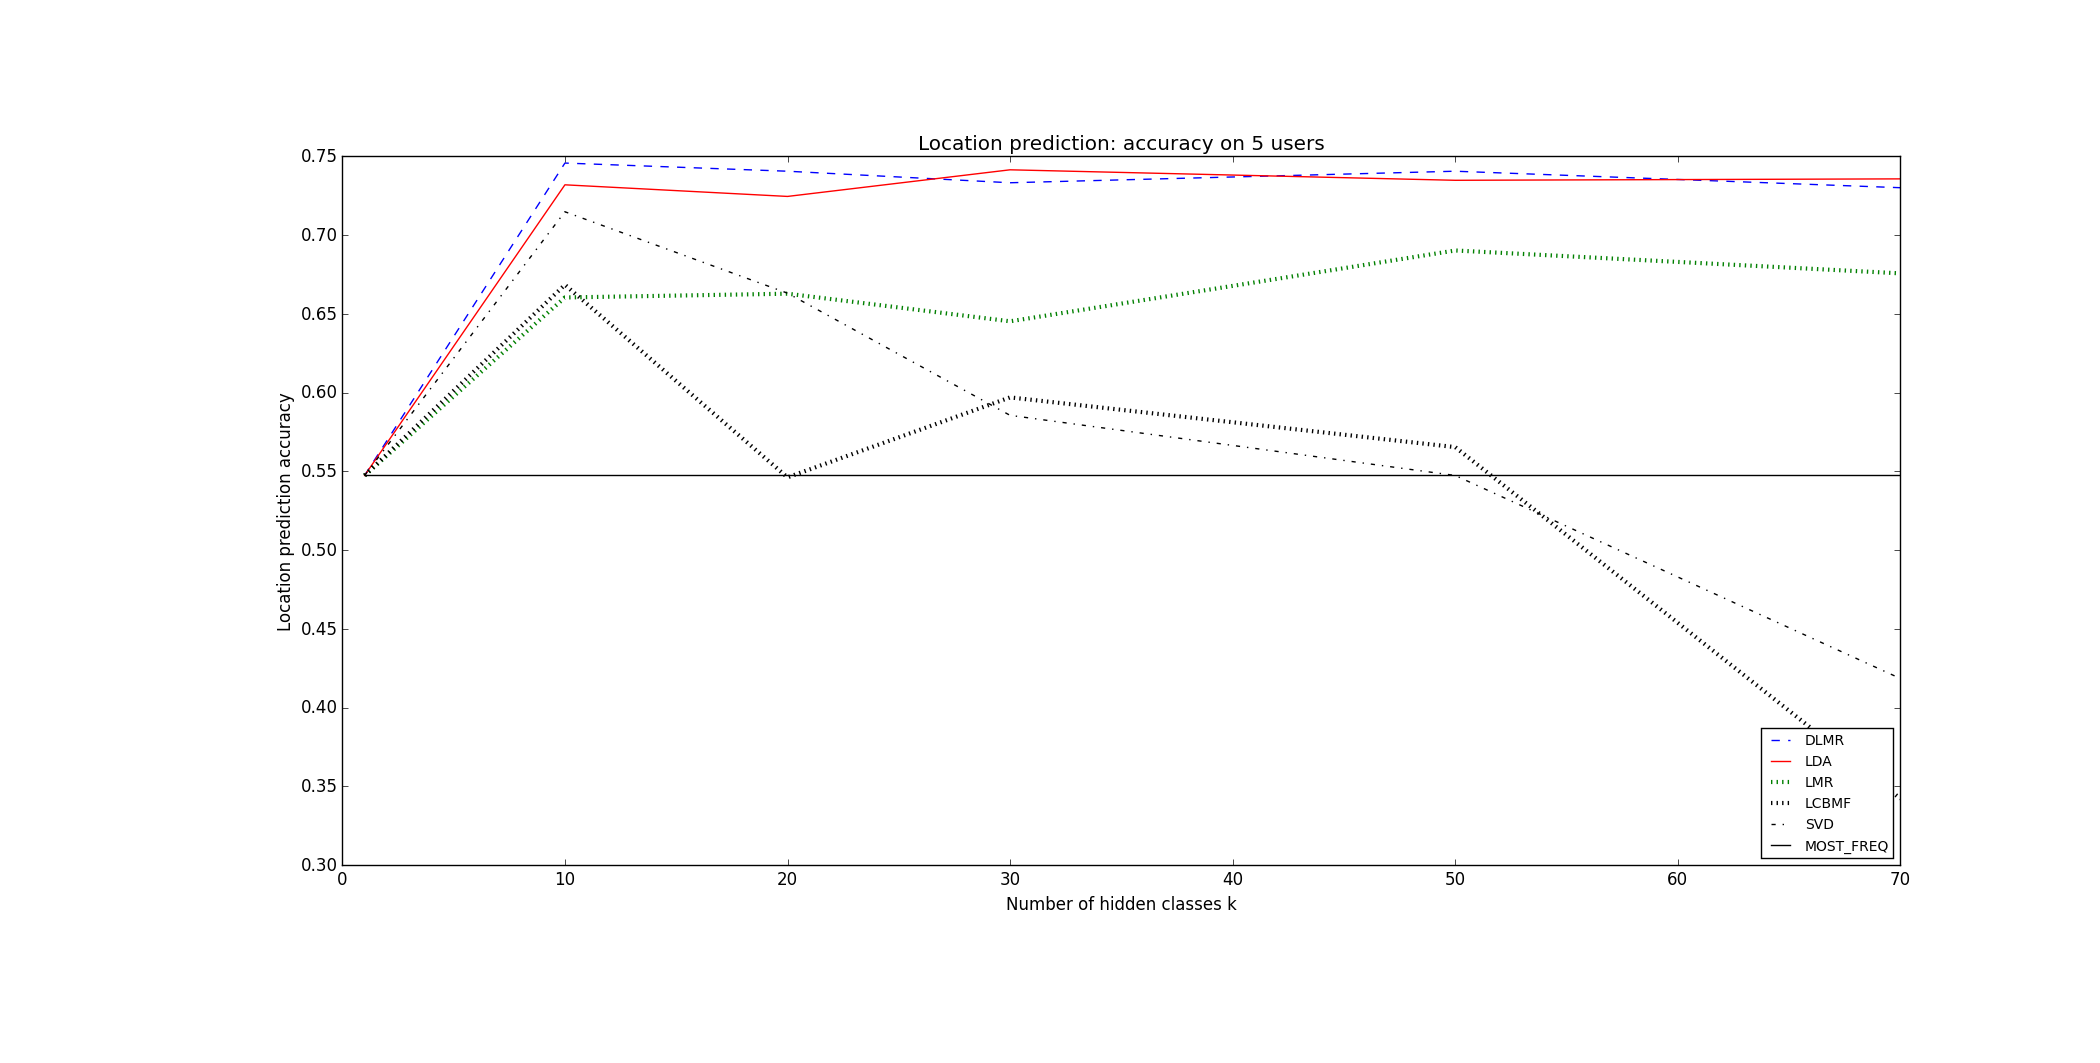
\includegraphics[scale=0.3]{Figures/location_accuracy.png}
\caption{Accuracy results of the prediction of the five models.}
\label{acc}
\end{figure}

\begin{figure} [!ht]
\centering
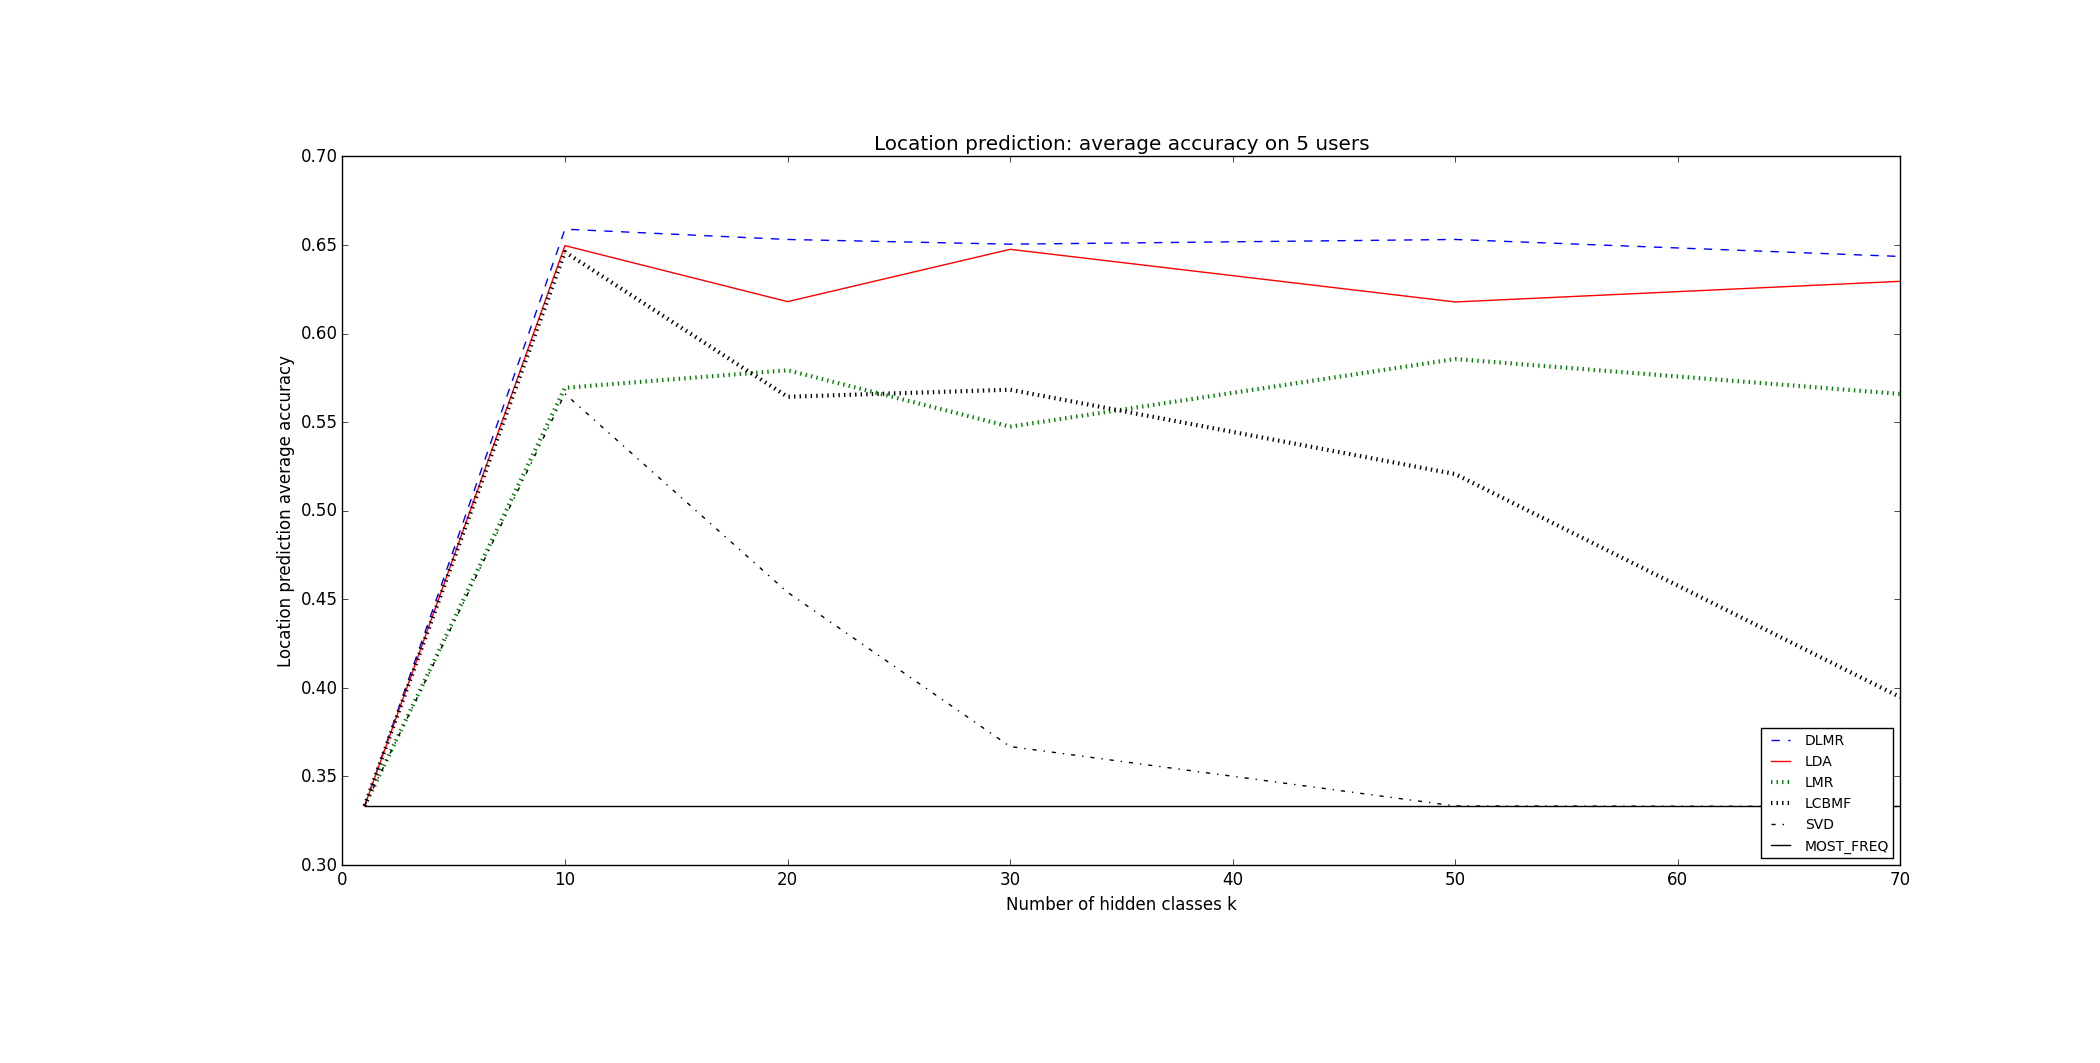
\includegraphics[scale=0.3]{Figures/location_average_accuracy.png}
\caption{Average accuracy results of the prediction of the five models.}
\label{avacc}
\end{figure}

First, we can see that the three probabilistic models, $DLMR$, $LDA$ and $LMR$ perform widely better than the matrix factorization models $LCBMF$ and $SVD$.
\\Indeed, when the number of behaviors increases ($K\geqslant 10$) the performance of $SVD$ and $LCBMF$ decreases heavily whereas $DLMR$ $LDA$ and $LMR$ stay relatively stable. This might be due to an effect of overfitting. \par

Deepen our observation int the three probabilistic models, we can see that $DLMR$ largely outperforms $LMR$. Indeed, the prediction scores of $DLMR$ are about 10\% better than $LMR$ for both average accuracy and accuracy for all the number of behaviors K. This confirms the intuition developed in chapter 3. While $LMR$ learns the behaviors expressed specifically by the records seen, $DLMR$ tries to catch a more general structure of the corpus by learning how the seen records generate the behaviors. This allows $DLMR$ to describe better an unseen data. Moreover, while both models show good stability to high number of behaviors, we can observe that for $K\geqslant 50$, $LMR$ score start to decrease while $DLMR$ is still enough stable for  $K=70$. The average accuracy plot shows this effect (average accuarcy of $LMR$ decreased by 3\% between $K = 50$ and $K = 70$ while average accuracy of $DLMR$ decreased only by 1 \% between $K = 50$ and $K = 70$, which is more due to the randomness of the test and train set rather than to overfitting). The same effect is present in the accuracies plots. 
\\As explained in chapter 3, $DLMR$ has $K+I$ ($I$ is the size of the language and equals $\sum_{f=1}^{J} I_f$) parameters to estimate while $LMR$ has $KM + KV$ parameters. Thus, when K increases the number of parameters to estimate increases much faster in $LMR$ than in $DLMR$. This is what might explain the observed effect in the sense that the big number of parameters in $LMR$ caused overfitting. \par

Concerning $LDA$, we see that it is also strong to overfitting (and stronger than $LMR$) and accurate in predictions. In fact, $LDA$ underlies the same properties than $DLMR$ (learn how records generate behaviors, small number of parameters to estimate). This is what explains its performance. However, $DLMR$ performs better than $LDA$ in prediction scores. Indeed, while they perform very close, $DLMR$ performs better than $LDA$ in average accuracy while keeping a similar score (or even slightly better score) to $LDA$ in $accuracy$. This means that $DLMR$ is able to better guess less frequent categories without loosing in general accuracy. This implies that $DLMR$ is better in detecting the rare events or contexts. This is explained by the structure of the model of $DLMR$. $DLMR$ imposes the probabilities of the values belonging to the same feature to sum to 1. This represents a much more realistic approximation of the real life than $LDA$ that spreads the probabilities over the space of all possible realizations. While frequent contexts (or events) can be outlined by an acceptable model of the real life, detecting rare contexts requires a much more precise representation.
\\Finally, evaluating $DLMR$ performance independently, we see that it performs around 74\% of good guesses and 67\% of average good guesses per class. This is a good prediction performance that shows that $DLMR$ is able to predict the future actions that the user might take. This implies that $DLMR$ was able to represent and learn the general behaviors according to which a user behaves.

As a sum up, the results show that the probabilistic models developed perform better in guessing right behaviors of users than the matrix factorization models exposed. Comparing the three probabilistic models $DLMR$, $LMR$ and $LDA$, $DLMR$ shows better results than both $LMR$ and $LDA$. This confirms the intuitions developed in chapter 3 that led us to the $DLMR$ model. Finally, the accuracies rate of $DLMR$ shows good generalization performance of unseen data, and thus proves that $DLMR$ is able to discover user behaviors from their logs.


%----------------------------------------------------------------------------------------
%	SECTION 3
%----------------------------------------------------------------------------------------

\section{Feature prediction results}
We recall that the final goal that drives our work is to discover the particular behaviors of a user from his smartphone logs. In this concluding section, we close the circle by showing examples of behaviors of the $5$ users discovered by $DLMR$. \par

First of all, and as one might expect, the $5$ users exhibit behavior that are similar. Indeed, there is at least one behavior for each user representing the fact that the user works in the week days during the day. There is also others expressing the fact that users are more often at home during the weekends, and others indicating that the users are almost always at home during the night (for all the days). An example of each of these $3$ behaviors is shown for one of the users in figure~\ref{commonBehavior} . 
\\However, one could have supposed those behaviors without analyzing smartphone logs. For this reason, they are not the most interesting habits that we aim to discover. We present them here for two reasons. First, it is a way to verify that $DLMR$ was able to discover some a-priori expected behaviors (as if we label users with some behaviors and then check that $DLMR$ is able to discover them). Second, we present them to give an intuition on how exactly the behaviors are represented in $DLMR$. \par

Now, we pay attention to examples of behaviors that are more interesting in the sense that they describe a specific user's habit. For example, the behavior in figure~\ref{readSunday} shows that $user1$ likes to do some readings on Sundays night. Indeed, $Reader$ (\href{https://play.google.com/store/apps/details?id=com.sony.drbd.reader.ext.pictorial.ja&hl=fr}{link}) is the package name of a Japanese smartphone application for purchasing and reading books. Alternatively, $user1$ would play $monster$ $strike$ (\href{https://play.google.com/store/apps/details?id=jp.co.mixi.monsterstrikeUS&hl=fr}{link}) or browse in the web using his smartphone ($Boat$ $Browser$ is the package name of a web browser (\href{https://play.google.com/store/apps/details?id=com.boatbrowser.free&hl=fr}{link})). 
\\The behavior in figure~\ref{news} shows that when the $user4$ is not at work during the day (in the week days), he would probably reads some news or watch some TV program. Indeed $SmartNews$ (\href{https://play.google.com/store/apps/details?id=jp.gocro.smartnews.android}{link}), $Socialife News$ (\href{https://play.google.com/store/apps/details?id=com.sony.nfx.app.sfrc&hl=fr}{link}) and $Gunosy$ (\href{https://play.google.com/store/apps/details?id=com.gunosy.android.world}{link}) are all news applications while $TV SideView Sony$ (\href{https://play.google.com/store/apps/details?id=com.sony.tvsideview.phone&hl=fr}{link}) is a smartphone TV app.
\\Finally, we end our example review with the behavior in figure~\ref{ing} . It shows that $user2$ is often playing ingress while being in $other$ $places$ during the weekends (in the day). In fact, $Ingress$ (l\href{https://play.google.com/store/apps/details?id=com.nianticproject.ingress&hl=fr}{link}) is an augmented reality playing location based game. In other terms, ingress is a game that transforms the real world in a game map, where players go from one place to the other trying to solve challenges. That's what explains the behavior of $user2$. \par

All these examples show that $DLMR$ is able to discover user's behaviors from his smartphone logs. In other terms, it is able to decompose a user's life (smartphone logs are a subsample of user's life) as a set of behaviors that are driving his life. Moreover, it is able to do so by extracting both general behaviors (as sleeping at home, working in the day) and more specific habits (reading on Sundays night, playing ingress on the week end). \par

Let's take a step back and recall the initial wish that led us to try to discover users' habbits. We wanted to enable smartphones to build a personal relationship with their owner by learning to know their habits and reacting to their specific needs. Thus we conclude this part by showing how the examples discussed above could be turned out to that end. For example, the smartphone of $user1$ could suggests to him new trendy books to read on Sundays night (even if $user1$ was not planning to read, maybe because he is bored with the books he is currently reading), or even proposes new games that he could play. Concerning $user2$, if his smartphone knows that it will be rainy next Sunday, then it could alert it's owner and suggests him to schedule his ingress session in another day if he is planning to play. Those are only few examples of possible applications and are far from being exhaustive. The work developed in this thesis does not already enable smartphones to act as described (smartphones need to be able to interpret the behaviors they extracted to do so), but allowing them to catch users' behaviors is a necessary and important step towards that direction.

\begin{figure*}[t!]
    \centering
    \begin{subfigure}[t]{0.33\textwidth}
        \centering
        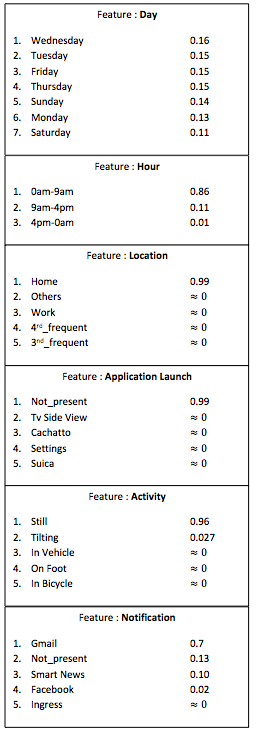
\includegraphics[scale=0.5]{Figures/Home.png}
        \caption{Home\_night.}
    \end{subfigure}%
    \begin{subfigure}[t]{0.33\textwidth}
        \centering
        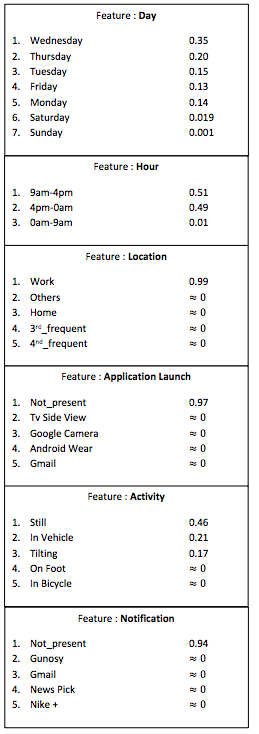
\includegraphics[scale=0.5]{Figures/Work.png}
        \caption{Working\_week\_days.}
    \end{subfigure}%
  \begin{subfigure}[t]{0.33\textwidth}
        \centering
        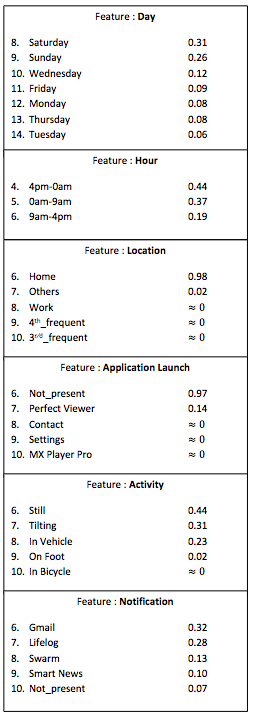
\includegraphics[scale=0.515]{Figures/Homeweekend.png}
        \caption{Home\_weekend.}
    \end{subfigure}

    \caption{Examples of common behaviors.}
\label{commonBehavior}
\end{figure*}


\begin{figure*}[t!]
    \centering
    \begin{subfigure}[t]{0.33\textwidth}
        \centering
        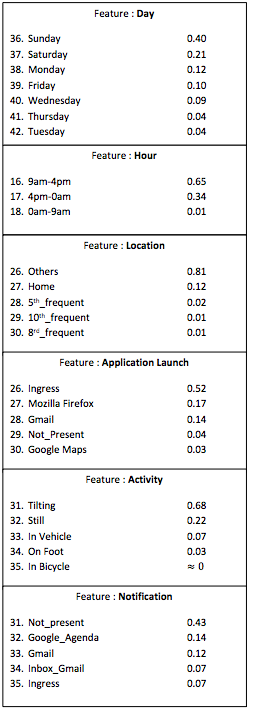
\includegraphics[scale=0.51]{Figures/Ingress.png}
        \caption{play\_ingress\_weekend.}
\label{ing}
    \end{subfigure}%
    \begin{subfigure}[t]{0.33\textwidth}
        \centering
        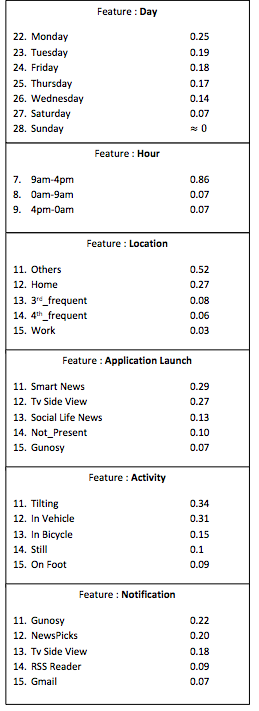
\includegraphics[scale=0.51]{Figures/News.png}
        \caption{Reading\_news\_mornings.}
\label{news}
    \end{subfigure}%
  \begin{subfigure}[t]{0.33\textwidth}
        \centering
        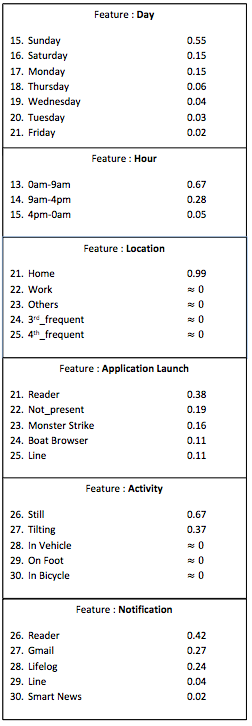
\includegraphics[scale=0.5]{Figures/sundayReading.png}
        \caption{reading\_sunday\_night.}
\label{readSunday}
    \end{subfigure}
    \caption{Examples of special behaviors.}
\label{specialBehavior}

\end{figure*}

 
% Chapter Template

\chapter{Conclusion} % Main chapter title

\label{Chapter7} % Change X to a consecutive number; for referencing this chapter elsewhere, use \ref{ChapterX}

\lhead{Chapter 7. \emph{Conclusion}} % Change X to a consecutive number; this is for the header on each page - perhaps a shortened title

In this work, we have described $Dirichlet$ $Latent$ $Multimodal$ $Representation$ ($DLMR$), a flexible generative probabilistic model for multimodal data (i.e data containing multiple types). $DLMR$ treats the different types of data separately by representing them in different distributions and in the same time combine them to underline common meaning expressed by these different types. We applied this model to smartphone logs dataset to extract behaviors of individual users from their logs.
In this work, our goal was to develop a model that enables extracting user's behaviors and habits from his smartphone logs (and to see how well this can be done).
\\To that end we developed a model that can specifically fit a multimodal data (i.e a data that contains multiple types) by treating each type separately and in the same time combining the different types to discover common relations expressed by the data. We called this model the $Dirichlet$ $Latent$ $Multimodal$ $Representation$ ($DLMR$).
\\We compared $DLMR$ to a complete overview of state of the art methods that could accomplish the same task. In this sense, we both considered matrix factorization approaches and probabilistic modeling approaches.
\\The results obtained show that $DLMR$ performs better than these models and in particular better than $Latent$ $Dirichlet$ $Allocation$ ($LDA$) and $Linearly$ $Constrained$ $Bayesian$ $Matrix$ $Factorization$ ($LCBMF$). Moreover, $DLMR$ shows good performances in discovering both general habits and specific behaviors of users based on their smartphones logs. \par

During this work, the need of developing $DLMR$ came from the specificity of the dataset we are considering. Indeed, while existing models are built to fit homogenous datasets containing only one type of information, $DLMR$ came from the need of modeling the heterogeneity of the smartphone logs dataset.
\\However, smartphone logs is not the only kind of dataset that has these characteristics. On the contrary, with the exponential increase of applications and platforms accessing to web, the rise of objects connected to the internet (sensor equipped cars, gym equipment machines) and the rapid growth of wearable devices (smart watch, smart glasses) and mobile mini-computers, datasets contains more and more multiple types of data. Because it was built by essence to model the multimodality of data, $DLMR$ can be applied to all these kind of datasets because and can be used for different purposes. It can for example be used to give a meaning to a non intuitive dataset, to predict future events, to classify data elements or to compress the size of a large dataset.

 
%\input{Chapters/Chapter6} 
%\input{Chapters/Chapter7} 

%----------------------------------------------------------------------------------------
%	THESIS CONTENT - APPENDICES
%----------------------------------------------------------------------------------------

\addtocontents{toc}{\vspace{2em}} % Add a gap in the Contents, for aesthetics

\appendix % Cue to tell LaTeX that the following 'chapters' are Appendices

% Include the appendices of the thesis as separate files from the Appendices folder
% Uncomment the lines as you write the Appendices

% Appendix A

\chapter{Appendix Title Here} % Main appendix title

\label{AppendixA} % For referencing this appendix elsewhere, use \ref{AppendixA}

\lhead{Appendix A. \emph{Appendix Title Here}} % This is for the header on each page - perhaps a shortened title

Write your Appendix content here.
%\input{Appendices/AppendixB}
%\input{Appendices/AppendixC}

\addtocontents{toc}{\vspace{2em}} % Add a gap in the Contents, for aesthetics

\backmatter

%----------------------------------------------------------------------------------------
%	BIBLIOGRAPHY
%----------------------------------------------------------------------------------------

\label{Bibliography}

\lhead{\emph{Bibliography}} % Change the page header to say "Bibliography"

\bibliographystyle{unsrtnat} % Use the "unsrtnat" BibTeX style for formatting the Bibliography

\bibliography{./Bibliography.bib} % The references (bibliography) information are stored in the file named "Bibliography.bib"

\end{document}  